% General
\documentclass[xcolor=table,aspectratio=169]{beamer}
\usetheme{Madrid}

% Figures
\usepackage{epsfig}
\usepackage{psfrag}
\usepackage{wrapfig}
\usepackage{graphicx}
\usepackage{subcaption}

% Colours
\usepackage{color}
\usepackage[table]{xcolor}
% Definitions of colours used in seaborn for use in latex
\definecolor{seaborn_bg_grey}{HTML}{eaeaf2}
\definecolor{seaborn_bg_grey_dark}{HTML}{d2d2d9}
\definecolor{seaborn_bg_grey_darker}{HTML}{a3a3a9}
\definecolor{seaborn_bg_grey_half}{HTML}{f4f4f8}

\definecolor{seaborn_blue}{HTML}{4c72b0}
\definecolor{seaborn_green}{HTML}{55a868}
\definecolor{seaborn_red}{HTML}{c44e52}
\definecolor{seaborn_magenta}{HTML}{8172b2}
\definecolor{seaborn_yellow}{HTML}{ccb974}
\definecolor{seaborn_cyan}{HTML}{64b5cd}

\definecolor{seaborn_muted_blue}{HTML}{4878cf}
\definecolor{seaborn_muted_green}{HTML}{6acc65}
\definecolor{seaborn_muted_red}{HTML}{d65f5f}
\definecolor{seaborn_muted_magenta}{HTML}{b47cc7}
\definecolor{seaborn_muted_yellow}{HTML}{c4ad66}
\definecolor{seaborn_muted_cyan}{HTML}{77bedb}

\definecolor{seaborn_pastel_blue}{HTML}{92c6ff}
\definecolor{seaborn_pastel_green}{HTML}{97f0aa}
\definecolor{seaborn_pastel_red}{HTML}{ff9f9a}
\definecolor{seaborn_pastel_magenta}{HTML}{d0bbff}
\definecolor{seaborn_pastel_yellow}{HTML}{fffea3}
\definecolor{seaborn_pastel_cyan}{HTML}{b0e0e6}

\definecolor{seaborn_bright_blue}{HTML}{003fff}
\definecolor{seaborn_bright_green}{HTML}{03ed3a}
\definecolor{seaborn_bright_red}{HTML}{e8000b}
\definecolor{seaborn_bright_magenta}{HTML}{8a2be2}
\definecolor{seaborn_bright_yellow}{HTML}{ffc400}
\definecolor{seaborn_bright_cyan}{HTML}{00d7ff}

\definecolor{seaborn_dark_blue}{HTML}{001c7f}
\definecolor{seaborn_dark_green}{HTML}{017517}
\definecolor{seaborn_dark_red}{HTML}{8c0900}
\definecolor{seaborn_dark_magenta}{HTML}{7600a1}
\definecolor{seaborn_dark_yellow}{HTML}{b8860b}
\definecolor{seaborn_dark_cyan}{HTML}{006374}

\definecolor{seaborn_colorblind_blue}{HTML}{0072b2}
\definecolor{seaborn_colorblind_green}{HTML}{009e73}
\definecolor{seaborn_colorblind_red}{HTML}{d55e00}
\definecolor{seaborn_colorblind_magenta}{HTML}{cc79a7}
\definecolor{seaborn_colorblind_yellow}{HTML}{f0e442}
\definecolor{seaborn_colorblind_cyan}{HTML}{56b4e9}


\definecolor{twitter_blue}{HTML}{1da1f2}
\definecolor{gruvbox_dark_bg}{HTML}{282828}
\definecolor{gruvbox_fg}{HTML}{ebdbb2}
\definecolor{kgrey}{HTML}{2b2828}
\definecolor{linh_pink}{HTML}{fd26ea}
\definecolor{linh_blue}{HTML}{2D8AC3}

% Fonts
\usepackage{amssymb}
\usepackage{amsmath}
\usepackage[T1]{fontenc}
\usepackage{pifont}
\usepackage{helvet}
\usepackage{cancel} % for \cancel
\usepackage[normalem]{ulem} % for \sout (strike out)
\renewcommand{\ttdefault}{pcr} % enables bold fixed width font

% Tables
\usepackage{array}
\usepackage{multicol}
\usepackage{tabularx}
\usepackage{multirow}
\newcolumntype{L}{>{\raggedright\arraybackslash}X}
\newcolumntype{C}{>{\centering\arraybackslash}X}
\newcolumntype{R}{>{\raggedleft\arraybackslash}X}
\usepackage{siunitx,booktabs}

% References
\usepackage[style=verbose-note, sorting=none, sortcites=true, maxnames=1, giveninits=true, autocite=superscript, doi=false, url=false, isbn=false, backend=biber, citetracker=false, pagetracker=false, bibencoding=utf8, eprint=false]{biblatex}
% Gobbling first names
\AtEveryCitekey{%
   \clearfield{shorttitle}%
   \clearfield{month}%
   \clearfield{day}%
   \ifentrytype{article}{%
      \clearfield{title}%
   }{}
   }
% "blindfootcite" is the equivalent of "footcite" except the number marker does not appear
\newcommand\blfootcite[1]{%
  \begingroup
  \renewcommand\thefootnote{}\footnote{\hspace{-4ex}\cite{#1}}%
  \addtocounter{footnote}{-1}%
  \endgroup
}
\renewcommand*{\multicitedelim}{\textcolor{seaborn_bg_grey_darker}{\addsemicolon}}
\setbeamerfont{footnote}{size=\scriptsize}
\renewcommand\footnoterule{\kern-3pt \color{seaborn_bg_grey_darker}\hrule width \textwidth height 0.4pt \color{black} \kern 2.6pt}
\DeclareSourcemap{
  \maps[datatype=bibtex,overwrite=False]{
   \map{
     \step[fieldsource=journal,
           match={Journal of Chemical Theory and Computation},
           replace={JCTC}]
     \step[fieldsource=journal,
           match={Reviews of Modern Physics},
           replace={Rev. Mod. Phys.}]
     \step[fieldsource=journal,
           match={Reports on Progress in Physics},
           replace={Rep. Prog. Phys.}]
     \step[fieldsource=journal,
           match={Physical Review Letters},
           replace={Phys. Rev. Lett.}]
     \step[fieldsource=journal,
           match={Physical Review},
           replace={Phys. Rev.}]
     \step[fieldsource=journal,
           match={B - Condensed Matter and Materials Physics},
           replace={B}]
     \step[fieldsource=journal,
           match={Journal of Chemical Physics},
           replace={J. Chem. Phys.}]
     \step[fieldsource=journal,
           match={Annual Review of Materials Research},
           replace={Annu. Rev. Mater. Res.}]
   }
  }
}

\renewbibmacro{in:}{}
\DeclareFieldFormat{pages}{\mkfirstpage{#1}}
\beamertemplatenavigationsymbolsempty
\setbeamertemplate{bibliography item}[text]
\renewbibmacro{in:}{}
\AtEveryBibitem{\clearfield{title}}
\AtEveryBibitem{\clearfield{month}}
\AtEveryBibitem{\clearfield{pages}}
\DeclareNameAlias{default}{given-family}
\bibliography{references.bib}

% Tikz
\usepackage{tikz}
\usetikzlibrary{positioning,shapes,arrows,backgrounds,fit,calc,external,trees,tikzmark,fadings}
\tikzfading[name=fade bottom,top color=transparent!0, bottom color=transparent!100]
% \tikzexternalize[prefix=tikzfigures/]
\tikzstyle{dummy} = []
\tikzstyle{line} = [draw, thick, -latex']
\tikzstyle{headless_line} = [draw, thick, -]
\tikzstyle{default}    = [rectangle, text centered, rounded corners, text=black, font=\sffamily\footnotesize, align=center]
\tikzstyle{default_text}    = [rectangle, text width=10cm, text=black,anchor=north west, font=\sffamily]
\tikzstyle{boxwhite} = [default, fill=white, rounded corners=0.1cm]
\tikzstyle{cp}    = [default, fill=seaborn_blue, text=white, text width=2.8cm, minimum height=0.5cm]
\tikzstyle{pw}    = [cp, fill=seaborn_green]
\tikzstyle{wannier90}    = [cp, fill=seaborn_cyan]
\tikzstyle{bespoke}    = [cp, fill=seaborn_magenta]
\tikzstyle{observable}    = [cp, fill=seaborn_red]
\tikzset{
  -|-/.style={
    to path={
      (\tikztostart) -| ($(\tikztostart)!#1!(\tikztotarget)$) |- (\tikztotarget)
      \tikztonodes
    }
  },
  -|-/.default=0.5,
  |-|/.style={
    to path={
      (\tikztostart) |- ($(\tikztostart)!#1!(\tikztotarget)$) -| (\tikztotarget)
      \tikztonodes
    }
  },
  |-|/.default=0.5,
}
\newlength{\myyshift}
\setlength{\myyshift}{0.05cm}
\usetikzlibrary{calc}
\newlength{\myfigscale}
\setlength{\myfigscale}{0.3cm}
\usepackage{smartdiagram}
\usesmartdiagramlibrary{additions}
% For tikz diagrams with nodes appearing on each slide
\tikzset{
  invisible/.style={opacity=0},
  visible on/.style={alt={#1{}{invisible}}},
  alt/.code args={<#1>#2#3}{%
    \alt<#1>{\pgfkeysalso{#2}}{\pgfkeysalso{#3}} % \pgfkeysalso doesn't change the path
  },
}

% Color boxes
\usepackage{tcolorbox}
\tcbuselibrary{skins,hooks}
\tcbset{colframe=structure,fonttitle=\bfseries,beamer, clip upper, boxsep=0pt, sharp corners=all, no shadow, left skip=0pt, right skip=0pt, coltext=white}

% Misc
\usepackage{adjustbox}
\usepackage{verbatim}
\usepackage{cleveref}
\usepackage{lipsum}

% New commands
\newcommand{\bra}[1]{\langle #1|}
\newcommand{\braket}[2]{\langle #1|#2\rangle}
\newcommand{\braopket}[3]{\langle #1|#2|#3\rangle}
\newcommand{\ket}[1]{|#1\rangle}
\newcommand{\nline}{\nonumber \\}
\newcommand{\Trace}{\mathsf{Tr}}
\newcommand{\insertframeinfo}{\insertframenumber/\inserttotalframenumber}
\newcommand{\backupbegin}{
   \newcounter{finalframe}
   \setcounter{finalframe}{\value{framenumber}}
   \renewcommand{\insertframeinfo}{}
}
\newcommand{\backupend}{
   \setcounter{framenumber}{\value{finalframe}}
}

% Numbering
\numberwithin{equation}{section}
\AtBeginEnvironment{frame}{\setcounter{footnote}{0}}

% Code blocks
% N.B.
%  - frame must have [fragile]
%  - use \begin{onlyenv} not \only
%  - after a lot of mucking around, I created gruvbox_plain as another style
%    that exclusively uses gruvbox's bg and fg with no syntax highlighting
%  - use [autogobble] to remove leading indentations
% (taken from https://github.com/daveyarwood/gruvbox-pygments)
\usepackage{minted}
\usemintedstyle{gruvbox-dark}
\setminted[python]{bgcolor=gruvbox_dark_bg}
\setminted[json]{bgcolor=gruvbox_dark_bg}
\setminted[shell-session]{style=gruvbox_plain, bgcolor=gruvbox_dark_bg}

% Beamer colors
\setbeamercolor{frametitle}{bg=kgrey,fg=white}
\setbeamerfont{normal text}{family=helvet}
\setbeamerfont{local structure}{family=helvet}
\setbeamercolor*{author in head/foot}{bg=seaborn_blue}
\setbeamercolor*{logo in head/foot}{bg=seaborn_blue,fg=white}
\setbeamercolor*{title in head/foot}{bg=seaborn_blue,fg=kgrey}
\setbeamercolor*{date in head/foot}{bg=seaborn_blue,fg=white}
\setbeamercolor{title}{fg=kgrey}
\setbeamercolor{under headline}{bg=seaborn_red}
\setbeamercolor{footline}{bg=seaborn_blue}
\setbeamercolor{caption name}{fg=seaborn_blue}
\setbeamercolor{block title}{bg=kgrey,fg=white}
\setbeamercolor{block body}{bg=seaborn_bg_grey,fg=black}
\setbeamercolor{footnote}{fg=seaborn_bg_grey_darker}
\setbeamertemplate{blocks}[default]
\setbeamerfont*{title in head/foot}{size=\small}
\setbeamerfont*{date in head/foot}{size=\small}
\setbeamerfont*{institute}{size=\Large}
% Lists
\setbeamertemplate{itemize items}{\normalsize $\bullet$}
\setbeamercolor{description item}{fg=seaborn_blue}
\setbeamertemplate{enumerate items}[default]
\setbeamercolor{enumerate item}{fg=seaborn_blue}
\setbeamercolor{itemize item}{fg=seaborn_blue}
\setbeamercolor{itemize subitem}{fg=seaborn_blue}
\setbeamercolor{itemize subsubitem}{fg=seaborn_blue}
% Bibliography
\setbeamercolor*{bibliography entry title}{fg=seaborn_bg_grey_darker}
\setbeamercolor*{bibliography entry author}{fg=seaborn_bg_grey_darker}
\setbeamercolor*{bibliography entry location}{fg=seaborn_bg_grey_darker}
\setbeamercolor*{bibliography entry note}{fg=seaborn_bg_grey_darker}
\setbeamertemplate{bibliography item}[text]

% Frame title
\setbeamertemplate{frametitle}
{
  \vspace{-1pt}
  \begin{beamercolorbox}[wd=\paperwidth,ht=0.8cm]{frametitle}
   \hspace{0.05em}
   \begin{minipage}[c]{0.8\textwidth}
     \bf \insertframetitle

   \end{minipage}
   \hfill
   \begin{minipage}{0.15\textwidth}
   \begin{flushright}
   \scriptsize \textbf{Edward Linscott}
   
   {\raisebox{-0.15cm}{
\includegraphics[height=0.45cm]{logos/psi_white_on_transparent.png}}
   \textbf{|}\hspace{0.1cm}
   \raisebox{-0.02cm}{\textbf{\insertframeinfo}}}%
   \vspace{-0.1cm}
   \end{flushright}
   \end{minipage}
   \vspace{0.125cm}
  \end{beamercolorbox}%
}

% Title page
\setbeamertemplate{title page}
{
  \leavevmode%
  \vbox{%
  \vspace{-0.15\paperwidth}%
  \noindent\begin{tcolorbox}[enhanced,watermark graphics=photos/psi_in_mist_large.jpg, width=1.01\paperwidth, height=0.741\paperwidth, watermark zoom=1.0, grow to left by=0.05\paperwidth, frame hidden, coltext=kgrey]

  \vspace{0.26\paperwidth}

  \begin{minipage}{\textwidth}
  %  \begin{flushright}
  %  \includegraphics[height=0.05\textheight]{logos/logo_marvel_color_transparent.png}
  %  \hspace{0.1ex}
  %  \includegraphics[height=0.05\textheight]{logos/SNF_logo_standard_web_color_pos_e.png}
  %  % \hspace{0.01\textheight}
  %  % \includegraphics[height=0.05\textheight]{logos/black_cropped.eps}
  %  \hspace{0.1cm}\hbox{}
  % \end{flushright}

  \begin{center} 
  \LARGE
      
  \textbf{\inserttitle}

  \large
  \textbf{\insertsubtitle}
  \end{center}
  \end{minipage}
  \end{tcolorbox}

  \vspace{-3.7em}
  \begin{tcolorbox}[width=0.976\paperwidth, enhanced, colback=kgrey, grow to left by=0.035\paperwidth,]
  %  \begin{center}
  %  \footnotesize\bf\insertauthor\quad \raisebox{0.1ex}{|} \quad \insertshortinstitute\ \quad \raisebox{0.1ex}{|} \quad THEOS Group Meeting \quad \raisebox{0.1ex}{|} \quad \insertdate \quad \raisebox{0.1ex}{|} \quad \includegraphics[height=1.5ex]{logos/SNF_logo_standard_web_sw_neg_e.png} \ \ \includegraphics[height=1.5ex]{logos/logo_marvel_color_transparent_inverted.png}
  %  \end{center}
  \vspace{-0.7ex}
  \hfill \footnotesize\bf\insertauthor \hfill \raisebox{0.1ex}{|} \hfill \raisebox{-1.1ex}{
\includegraphics[height=3.4ex]{logos/psi_white_on_transparent.png}} \hfill \raisebox{0.1ex}{|} \hfill \insertdate \hfill \raisebox{0.1ex}{|} \hfill 
\includegraphics[height=1.5ex]{logos/snf_white_on_transparent.png} \ \ 
\includegraphics[height=1.5ex]{logos/marvel_white_on_transparent.png} \ \hfill
  %  \end{flushright}
  \end{tcolorbox}
  }
}
%\setbeamerfont{frametitle}{series=\bfseries}
\setbeamertemplate{footline}
{
}

% Title slide %%%%%%%%%%%%%%%%%%%%%%%%%%%%%%%%%%%%%%%%%%%%%%%%%%%%%%%%%%%%%%%%%%%%%%%%%%%%%%%%%%%
\author{Edward Linscott}
\institute{Laboratory for Materials Simulations\\Paul Scherrer Institute}
\date{24 April 2024}
\title{Koopmans functionals}
\subtitle{a brief introduction}

% Document contents
\begin{document}

% Title slide
\frame{\titlepage}

\begin{frame}{Koopmans functionals: theory}
   \begin{columns}
      \begin{column}{0.6\textwidth}
         \only<1-3>{%
         How can we calculate the energies of charged excitations? Why does DFT fail?

         \onslide<2-3>{%
         \vspace{1ex}%
         For the exact Green's function, we have poles that correspond to total energy differences
         \begin{equation*}
            \varepsilon_i =
            \begin{cases}
            E(N) - E_i(N-1) & i \in \text{occ} \\
            E_i(N+1) - E(N) & i \in \text{emp}
            \end{cases}
         \end{equation*}}

         \onslide<3>{%
         \vspace{1ex}
         For DFT, this condition is \emph{not} satisfied in general
         }}

         \only<4->{%
         \textbf{Core idea:} for every orbital $i$ their energy
         \begin{equation*}
            \varepsilon^\mathsf{Koopmans}_i = \braopket{\varphi_i}{H}{\varphi_i} = \partial E_\mathsf{Koopmans}/\partial f_i
         \end{equation*}
         ought to be...
         \begin{itemize}
            \item independent of its own occupation $f_i$
            \item equal to the corresponding total energy difference $E_i(N-1) - E(N)$
         \end{itemize}
         }
         \hfill
         %
      \end{column}
      \begin{column}{0.4\textwidth}
         \centering
            \only<1>{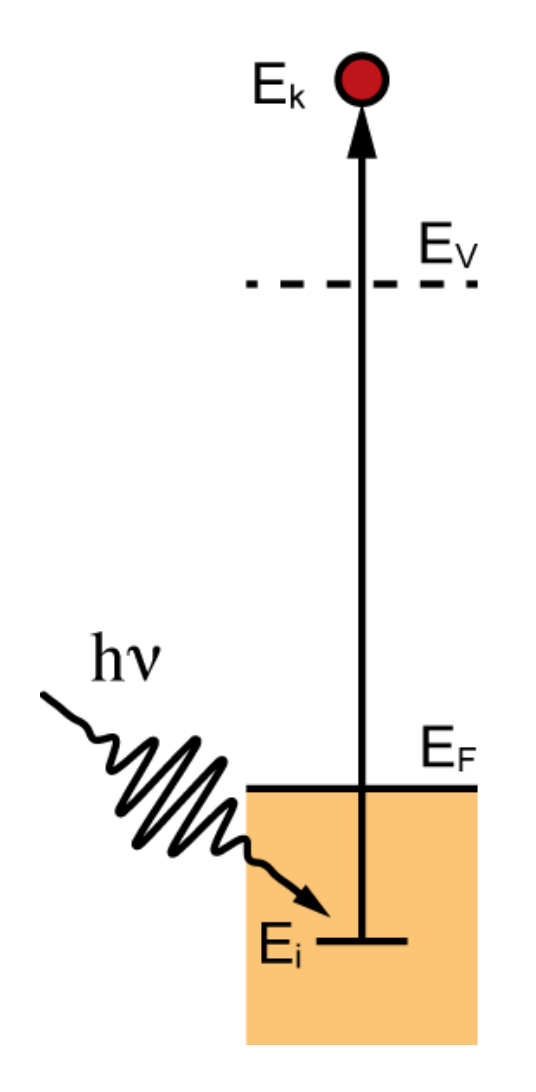
\includegraphics[height=0.5\textheight]{figures/photoemission_costantini.png}}
            \only<2->{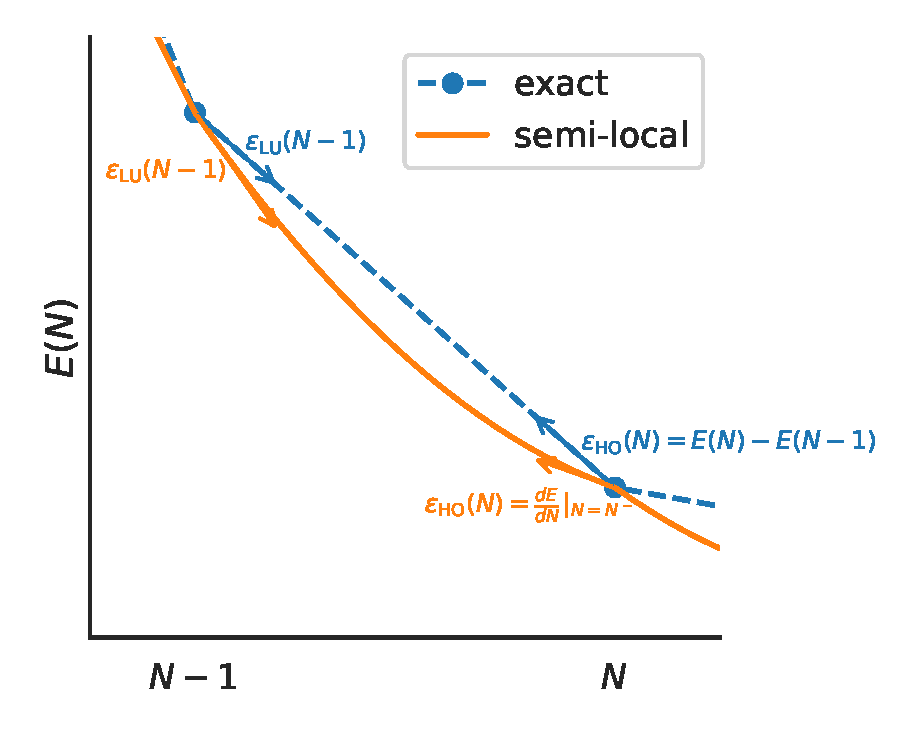
\includegraphics[width=\columnwidth]{figures/curvature_plot/fig_en_curve_gradients_zoom.pdf}}
      \end{column}
   \end{columns}
   \onslide<1>{\blfootcite{Costantini2020}}
\end{frame}

\begin{frame}{Koopmans functionals: theory}
   \begin{align*}
      E_\mathsf{KI}[\rho,\only<4>{\textcolor{red}}{\{\rho_i\}}, \only<3>{\textcolor{red}}{\{\alpha_i\}}]
      = \only<2>{\textcolor{red}}{E_\mathsf{DFT}[\rho]}
      \only<1-2>{
      + \sum_i
      \biggl( &\underbrace{
      -\left(E_\mathsf{DFT} -E_\mathsf{DFT}|_{f_i=0}\right)}_{\only<2>{\textcolor{red}}{\textsf{removes erroneous curvature}}}\nonumber                                                                                             \\
              & \qquad + \underbrace{f_i \left( E_\mathsf{DFT}|_{f_i=1} -E_\mathsf{DFT}|_{f_i=0} \right)}_{\only<2>{\textcolor{red}}{\textsf{restores linear behaviour}}}
      \biggr)
      }
      \only<3->{
      + \sum_i
      \only<3>{\textcolor{red}}
      {\alpha_i}
      \biggl( &\underbrace{
      E_\mathsf{Hxc} [\rho-\only<4>{\textcolor{red}}{\rho_i}] -E_\mathsf{Hxc}[\rho]}_{\only<2>{\textcolor{red}}{\textsf{removes erroneous curvature}}}\nonumber                                                                                             \\
              & \qquad + \underbrace{f_i \left( E_\mathsf{Hxc}[\rho-\only<4>{\textcolor{red}}{\rho_i}+\only<4>{\textcolor{red}}{n_i}] -E_\mathsf{Hxc}[\rho-\only<4>{\textcolor{red}}{\rho_i}] \right)}_{\only<2>{\textcolor{red}}{\textsf{restores linear behaviour}}}
      \biggr)
      }
   \end{align*}
   \onslide<2->{General features:}
   \begin{itemize}[<+(1)->]
      \item a correction to DFT that ensures eigenvalues match total energy differences
      \item to evaluate, requires the introduction of screening parameters $\alpha_i$ (replacing $E_\mathsf{DFT}|_{f_i=f}$ with $E_\mathsf{DFT}[\rho - \rho_i + f n_i]$)
      \item is orbital-density-dependent
   \end{itemize}

\end{frame}

\begin{frame}{Koopmans functionals: theory}
   Consequences of ODD:
   \begin{itemize}[<+(1)->]
      \item variational (localized, minimizing) vs canonical (delocalized, diagonalizing) orbitals
            \begin{figure}[t]
               \centering
               \begin{subfigure}{0.3\textwidth}
                  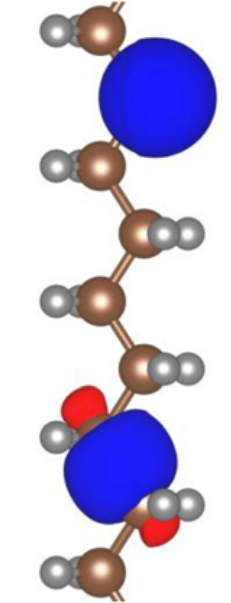
\includegraphics[height=\columnwidth,angle=90]{figures/fig_nguyen_variational_orbital.png}
                  \caption{variational}
               \end{subfigure}
               \hspace{0.1\textwidth}
               \begin{subfigure}{0.3\textwidth}
                  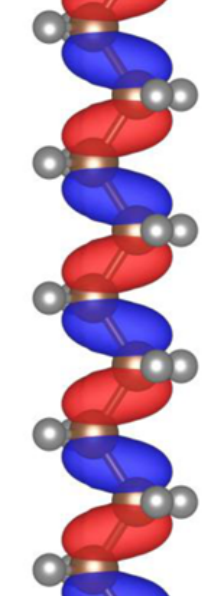
\includegraphics[height=\columnwidth,angle=90]{figures/fig_nguyen_canonical_orbital.png}
                  \caption{canonical}
               \end{subfigure}
            \end{figure}
      \item Practically we can often use MLWFs
      \item localized variational orbitals naturally allow us to treat bulk systems
      % \item ODD functional means that we know $\hat H \ket{\varphi_i}$ for variational orbitals $\{\ket{\varphi_i}\}$ but we don't know $\hat H$ in general
   \end{itemize}
   \blfootcite{Nguyen2018}
\end{frame}

\begin{frame}{Koopmans functionals: the bulk limit}

   \begin{center}
      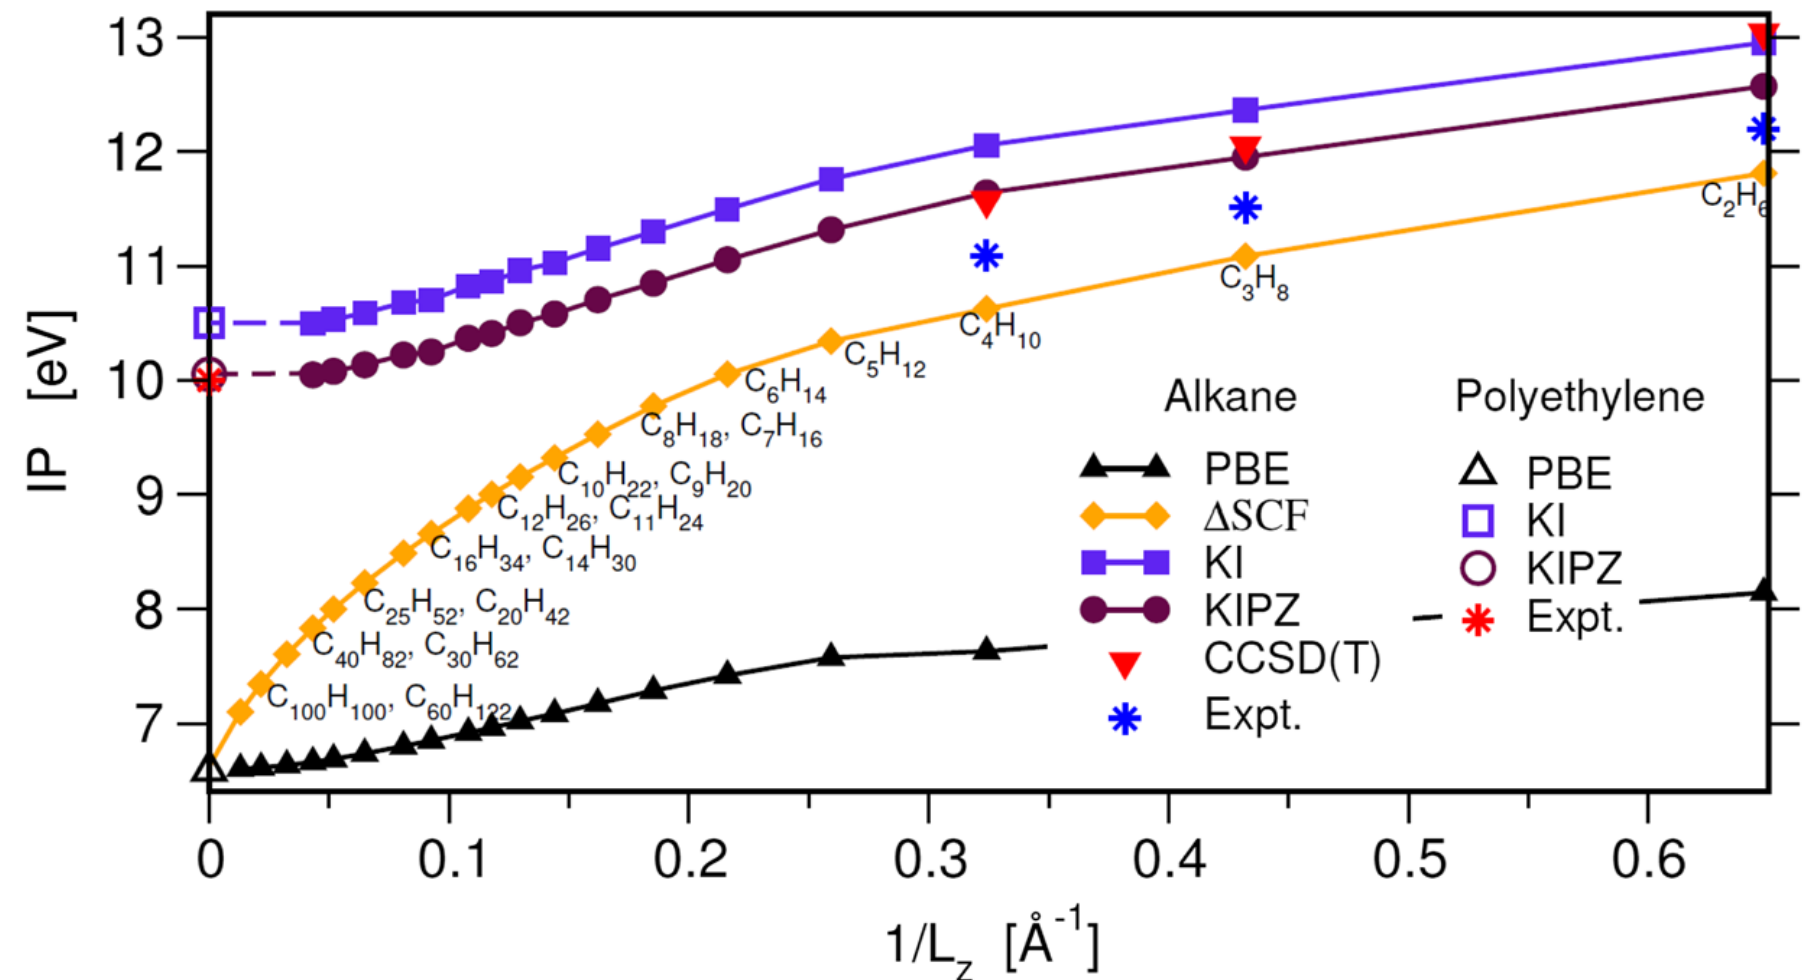
\includegraphics[width=0.6\textwidth]{figures/fig_nguyen_scaling.png}
   \end{center}
   \onslide<2->{
      \noindent In the bulk limit for one cell $\Delta E_\text{one cell} = E(N-\delta N) - E(N)$
   }%

   \onslide<3>{ 
      Across all the cells $
         \Delta E_\text{all cells} = \frac{1}{\delta N}\left(E(N-\delta N) - E(N)\right) = -\frac{dE}{dN} = -\varepsilon_\mathsf{HO}$
   }%

   \blfootcite{Nguyen2018}

\end{frame}


% \begin{frame}{Koopmans functionals: comparing}
%    \small
%    \renewcommand{\arraystretch}{1.5}
%    \rowcolors{1}{seaborn_bg_grey}{seaborn_bg_grey_half}
%    \begin{tabularx}{\columnwidth}{L L L}
%                                                 & \textbf{DFT+\emph{U}}                                                       & \textbf{Koopmans}                                                                                                                                                   \\
%       \hline
%       designed to correct SIE, as defined by... & erroneous global curvature in total energies                                & dependence of $\varepsilon_i$ on $f_i \ \forall i$ \leavevmode\onslide<4->{\textcolor{red}{(canonical orbitals)}}                                                   \\
%       by construction...                        & corrects local curvature in total energies                                  & removes dependence of $\varepsilon_i$ on $f_i$ and guarantees $\varepsilon_i = E_i(N\pm 1) - E(N)$ \leavevmode\onslide<4->{\textcolor{red}{(variational orbitals)}} \\
%       correction applied to...                  & selected subspaces only (e.g. \emph{3d} orbitals)                           & the entire system                                                                                                                                                   \\
%       orbitals defined by...                    & Hubbard projectors (atom-centred, frozen, incomplete)                       & \leavevmode\onslide<2->{variational (minimising) orbitals}                                                                                                          \\
%       corrective parameters are...              & $\{U^I\}$, defined with respect to charge-neutral excitations (if using LR) & \leavevmode\onslide<3->{$\{\alpha_i\}$, defined with respect to charged excitations}                                                                                \\
%    \end{tabularx}
% \end{frame}

\begin{frame}{Koopmans functionals: theory}
   Resonance with other efforts:
   \begin{itemize}
      \item Wannier transition-state method of Anisimov and Kozhevnikov \cite{Anisimov2005}
      \item Optimally tuned hybrid functionals of Kronik, Pasquarello, and others \cite{Kronik2012,Wing2021}
      \item Ensemble DFT of Kronik and co-workers \cite{Kraisler2013}
      \item Koopmans-Wannier of Wang and co-workers \cite{Ma2016}
      \item Dielectric-dependent hybrid functionals of Galli and co-workers \cite{Skone2016a}
      \item LOSC functionals of Yang and co-workers \cite{Li2018}
   \end{itemize}
\end{frame}

\begin{frame}{Koopmans functionals: results for molecules}
   \small
   Ionization potentials for the GW100 set cf. CCSD(T)
   \begin{center}
      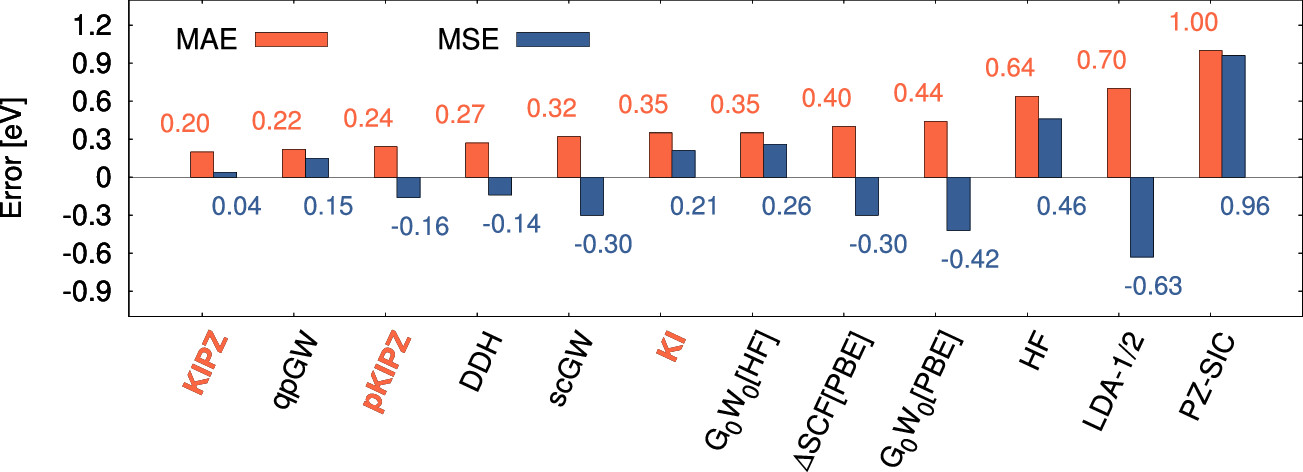
\includegraphics[height=0.2\textwidth]{figures/colonna_2019_gw100_ip}
      % \onslide<2->{\includegraphics[height=0.23\textwidth]{figures/colonna_2019_gw100_deeper}}
   \end{center}

   \vspace{-3ex}
   Ultraviolet photoemission spectra
   \begin{center}
      \begin{tikzpicture}
         \node [inner sep=0pt](fig) at (0,0) {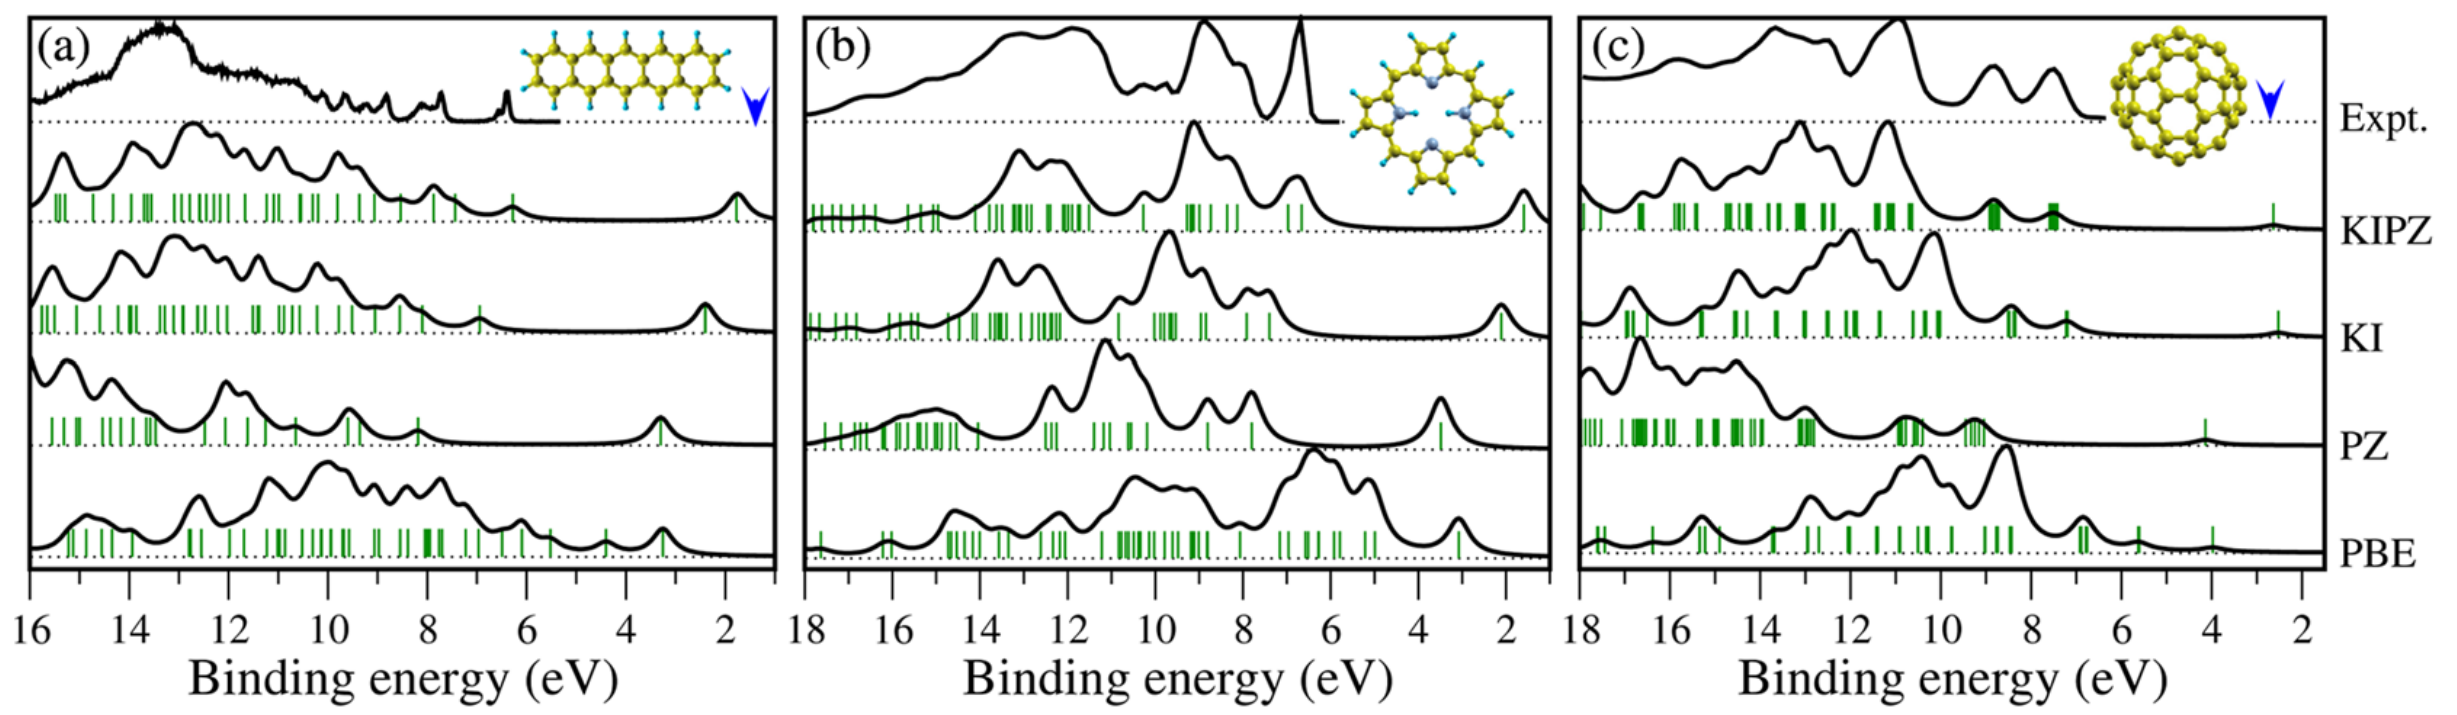
\includegraphics[height=0.35\textheight]{figures/fig_nguyen_prl_spectra.png}};
         \draw [very thick, color=seaborn_red] (-5.35,-0.07) rectangle (5.4,1.6);
      \end{tikzpicture}
   \end{center}
   \vspace{-2ex}

   \blfootcite{Colonna2018,Nguyen2015}
\end{frame}

% \begin{frame}{Koopmans functionals: results for molecules}
%    Electron affinities $ = E(N) - E(N+1) \stackrel{?}{=} -\varepsilon_{LU}$ of molecules cf. CCSD(T)/exp
%    \vspace{2ex}
% 
%    \small
%    \begin{center}
%       For 15 of the GW100 molecules with bound LUMOs
% 
%       \includegraphics[height=0.5\textheight]{figures/fig_gw100_ea_mae_mse.pdf}
% 
%       \textcolor{seaborn_bg_grey_darker}{\footnotesize Linscott et al. (in prep)}
%    \end{center}
% \end{frame}

\begin{frame}{Koopmans functionals: results for solids}
   \begin{minipage}[c]{0.35\textwidth}
      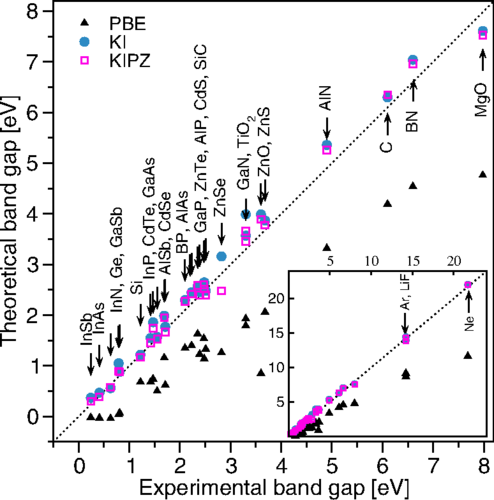
\includegraphics[width=\textwidth]{figures/fig_nguyen_prx_bandgaps.png}
   \end{minipage}
   \hspace{1em}
   \begin{minipage}[c]{0.6\textwidth}

      \footnotesize
      Mean absolute error (eV) across prototypical semiconductors and insulators

      \vspace{1ex}
      \begin{tabular}{c S[table-format = 2.2] S[table-format = 2.2] >{\color{seaborn_red}\bfseries}S[table-format = 2.2] >{\color{seaborn_red}\bfseries}S[table-format = 2.2] S[table-format = 2.2]}
                          & {PBE} & {G\textsubscript{0}W\textsubscript{0}} & {KI} & {KIPZ} & {QSG$\tilde{\mathsf{W}}$} \\
         \midrule
         \midrule
         $E_\mathsf{gap}$ & 2.54  & 0.56                                   & 0.27 & 0.22   & 0.18                      \\
         %                                  & {MAPE (\%)} & 48.28 & 12.10      & 7.0           \\
         \midrule
         IP               & 1.09  & 0.39                                   & 0.19 & 0.21   & 0.49                      \\
         %                                  & {MAPE (\%)} & 15.58 & 5.71                                   & 2.99 & 3.14   & 7.41
      \end{tabular}
   \end{minipage}

   \blfootcite{Nguyen2018}
\end{frame}

\begin{frame}{Koopmans functionals: results for solids}
   
\begin{table}[t]
   \centering
   \footnotesize
   \begin{tabular}{r@{ $\rightarrow$ } l *{3}{S[table-format = 2.2]} >{\color{seaborn_red}}S[table-format = 2.2] >{\color{seaborn_red}}S[table-format = 2.2] S[table-format = 2.2] @{$\pm$} S[table-format = 1.2]}
      \hline
      \hline
      \multicolumn{2}{c}{ }
                                & \multicolumn{1}{c}{PBE}
                                & \multicolumn{1}{c}{G\textsubscript{0}W\textsubscript{0}\footnote{\cite{Shishkin2007} for $E_g$ and \cite{Hybertsen1986} for the transitions;}}
                                & \multicolumn{1}{c}{scG$\tilde{\mathsf{W}}$\footcite{Shishkin2007a}}
                                & \multicolumn{1}{c}{
                                 \textcolor{seaborn_red}{\bfseries KI@[PBE,MLWFs]}}
                                & \multicolumn{1}{c}{
                                 \textcolor{seaborn_red}{\bfseries KIPZ@PBE}}
                                & \multicolumn{2}{c}{exp\footcite{Madelung2004}}                                                                                                                                                                   \\
      \hline
      \multicolumn{2}{c}{$E_g$} &
      0.49 &  1.06 & 1.14 &  1.16 &   1.15 & \multicolumn{2}{c}{1.17}\\
      $\Gamma_{1v}$ & $\Gamma_{25'v}$ & 11.97 & 12.04 &      & 11.97 & 12.09 & 12.5 &  0.6\\
      $X_{1v}$ & $\Gamma_{25'v}$ &  7.82 &       &      &  7.82       &       & \multicolumn{2}{c}{7.75}\\
      $X_{4v}$ & $\Gamma_{25'v}$ &  2.85 &  2.99 &      &  2.85 & 2.86 & \multicolumn{2}{c}{2.90}\\
      $L_{2'v}$ & $\Gamma_{25'v}$ &  9.63 &  9.79 &      &  9.63 &  9.74 &  9.3 &  0.4\\
      $L_{1v}$ & $\Gamma_{25'v}$ &  6.98 &  7.18 &      &  6.98 &   7.04 &  6.8 &  0.2\\
      $L_{3'v}$ & $\Gamma_{25'v}$ &  1.19 &  1.27 &      &  1.19 &       &  1.2 &  0.2\\
      $\Gamma_{25'v}$ &  $\Gamma_{15c}$ &  2.48 &  3.29 &      &  3.17  &  3.20 & 3.35 & 0.01\\
      $\Gamma_{25'v}$ &  $\Gamma_{2'c}$ &  3.28 &  4.02 &      &  3.95  &  3.95 & 4.15 & 0.05\\
      $\Gamma_{25'v}$ &        $X_{1c}$ &  0.62 &  1.38 &      &  1.28  &  1.31 & \multicolumn{2}{c}{1.13} \\
      $\Gamma_{25'v}$ &        $L_{1c}$ &  1.45 &  2.21 &      &  2.12  &  2.13 & 2.04 & 0.06\\
      $\Gamma_{25'v}$ &        $L_{3c}$ &  3.24 &  4.18 &      &  3.91  &  3.94 &  3.9 &  0.1\\
      \hline
      \multicolumn{2}{c}{MSE} & 0.35 &  0.02 &      &  0.01 &   0.03\\
      \multicolumn{2}{c}{MAE} & 0.44 &  0.21 &      &  0.14 &   0.17\\
      \hline
      \hline
   \end{tabular}

   % \textsuperscript{\emph{a}} this work;
   % \textsuperscript{\emph{b}} Ref.~\citenum{Shishkin2007} for $E_g$ and Ref.~\citenum{Hybertsen1986} for the transitions;
   % \textsuperscript{\emph{c}} Ref.~\citenum{Shishkin2007a};
   % \textsuperscript{\emph{d}} Ref.~\citenum{DeGennaro2022};
   % \textsuperscript{\emph{e}} Ref.~\citenum{Madelung2004}
\end{table}
\end{frame}


\begin{frame}{Koopmans functionals: caveats}

   \begin{itemize}[<+(1)->]
      \item restricted to systems with a non-zero band gap
      \item empty state localization in the bulk limit
      \item can potentially break the crystal point group symmetry\blfootcite{Su2020}
   \end{itemize}
\end{frame}


\begin{frame}{Recent improvements}
   The general workflow:
   \begin{itemize}
      \item initialize a set of variational orbitals
      \item calculate the screening parameters $\{\alpha_i\}$
      \item construct and diagonalize the Hamiltonian
   \end{itemize}

   Recent advances make some of these steps a lot easier...
\end{frame}

\begin{frame}{Recent improvements: easier Wannierization}

   \begin{figure}[t]
      \begin{subfigure}{0.225\textwidth}
         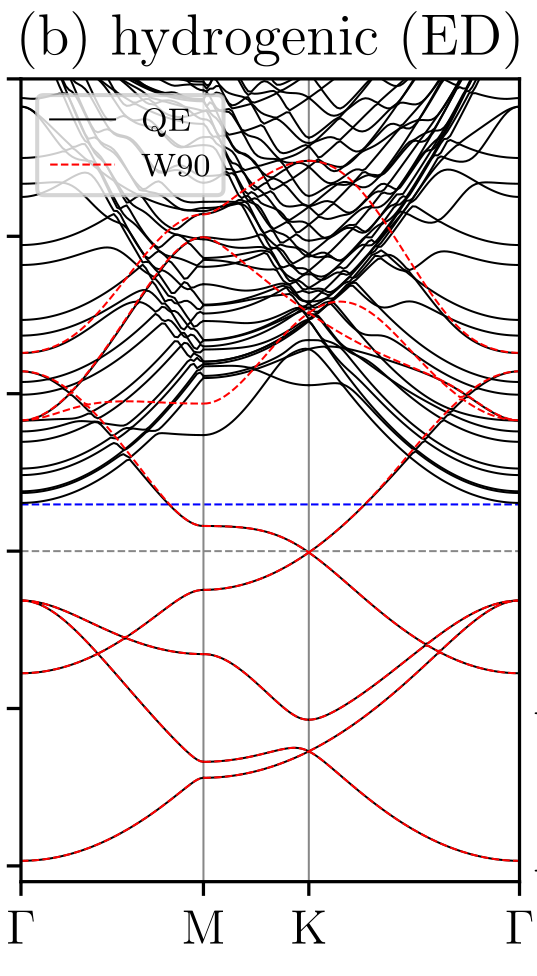
\includegraphics[height=1.5\columnwidth]{figures/proj_disentanglement_fig1b.png}
         \vspace{-0.01\paperheight}
      \end{subfigure}
      \begin{subfigure}{0.225\textwidth}
         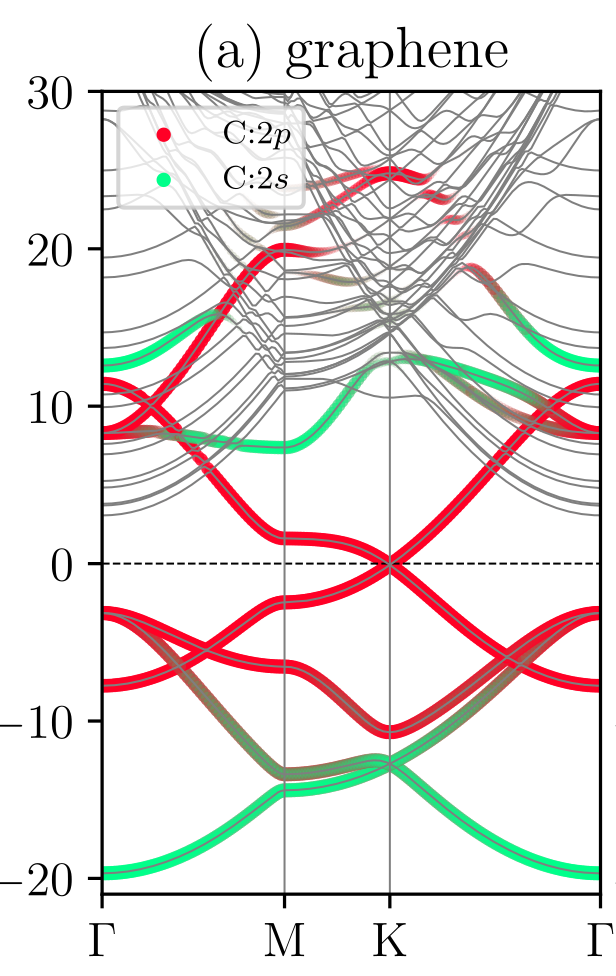
\includegraphics[height=1.5\columnwidth]{figures/proj_disentanglement_fig1a.png}
      \end{subfigure}
      \hspace{0.025\textwidth}
      % \begin{subfigure}{0.225\textwidth}
      %    \onslide<3->{
      %    \includegraphics[height=1.5\columnwidth]{figures/proj_disentanglement_fig1d.png}
      %    }
      % \end{subfigure}
      \begin{subfigure}{0.225\textwidth}
         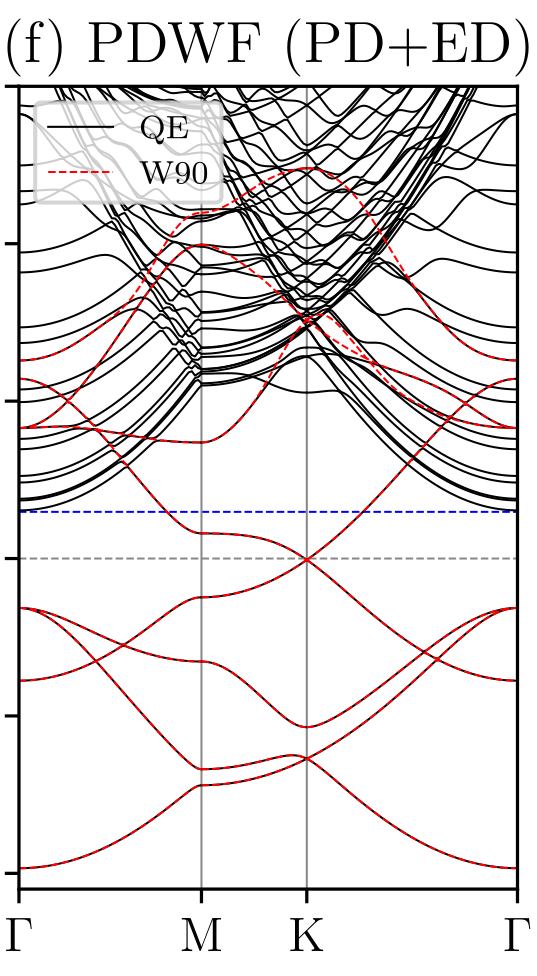
\includegraphics[height=1.5\columnwidth]{figures/proj_disentanglement_fig1f.png}
      \end{subfigure}
   \end{figure}

   \onslide<2->{Demonstrated on $>$20,000 materials $\rightarrow$ black-box Wannierization!}

   \blfootcite{Qiao2023}

\end{frame}

\begin{frame}{Recent improvements: easier Wannierization}
   Separation of target manifolds via parallel transport to obtain separate occupied and empty manifolds

      \begin{figure}
         \onslide<2->{
         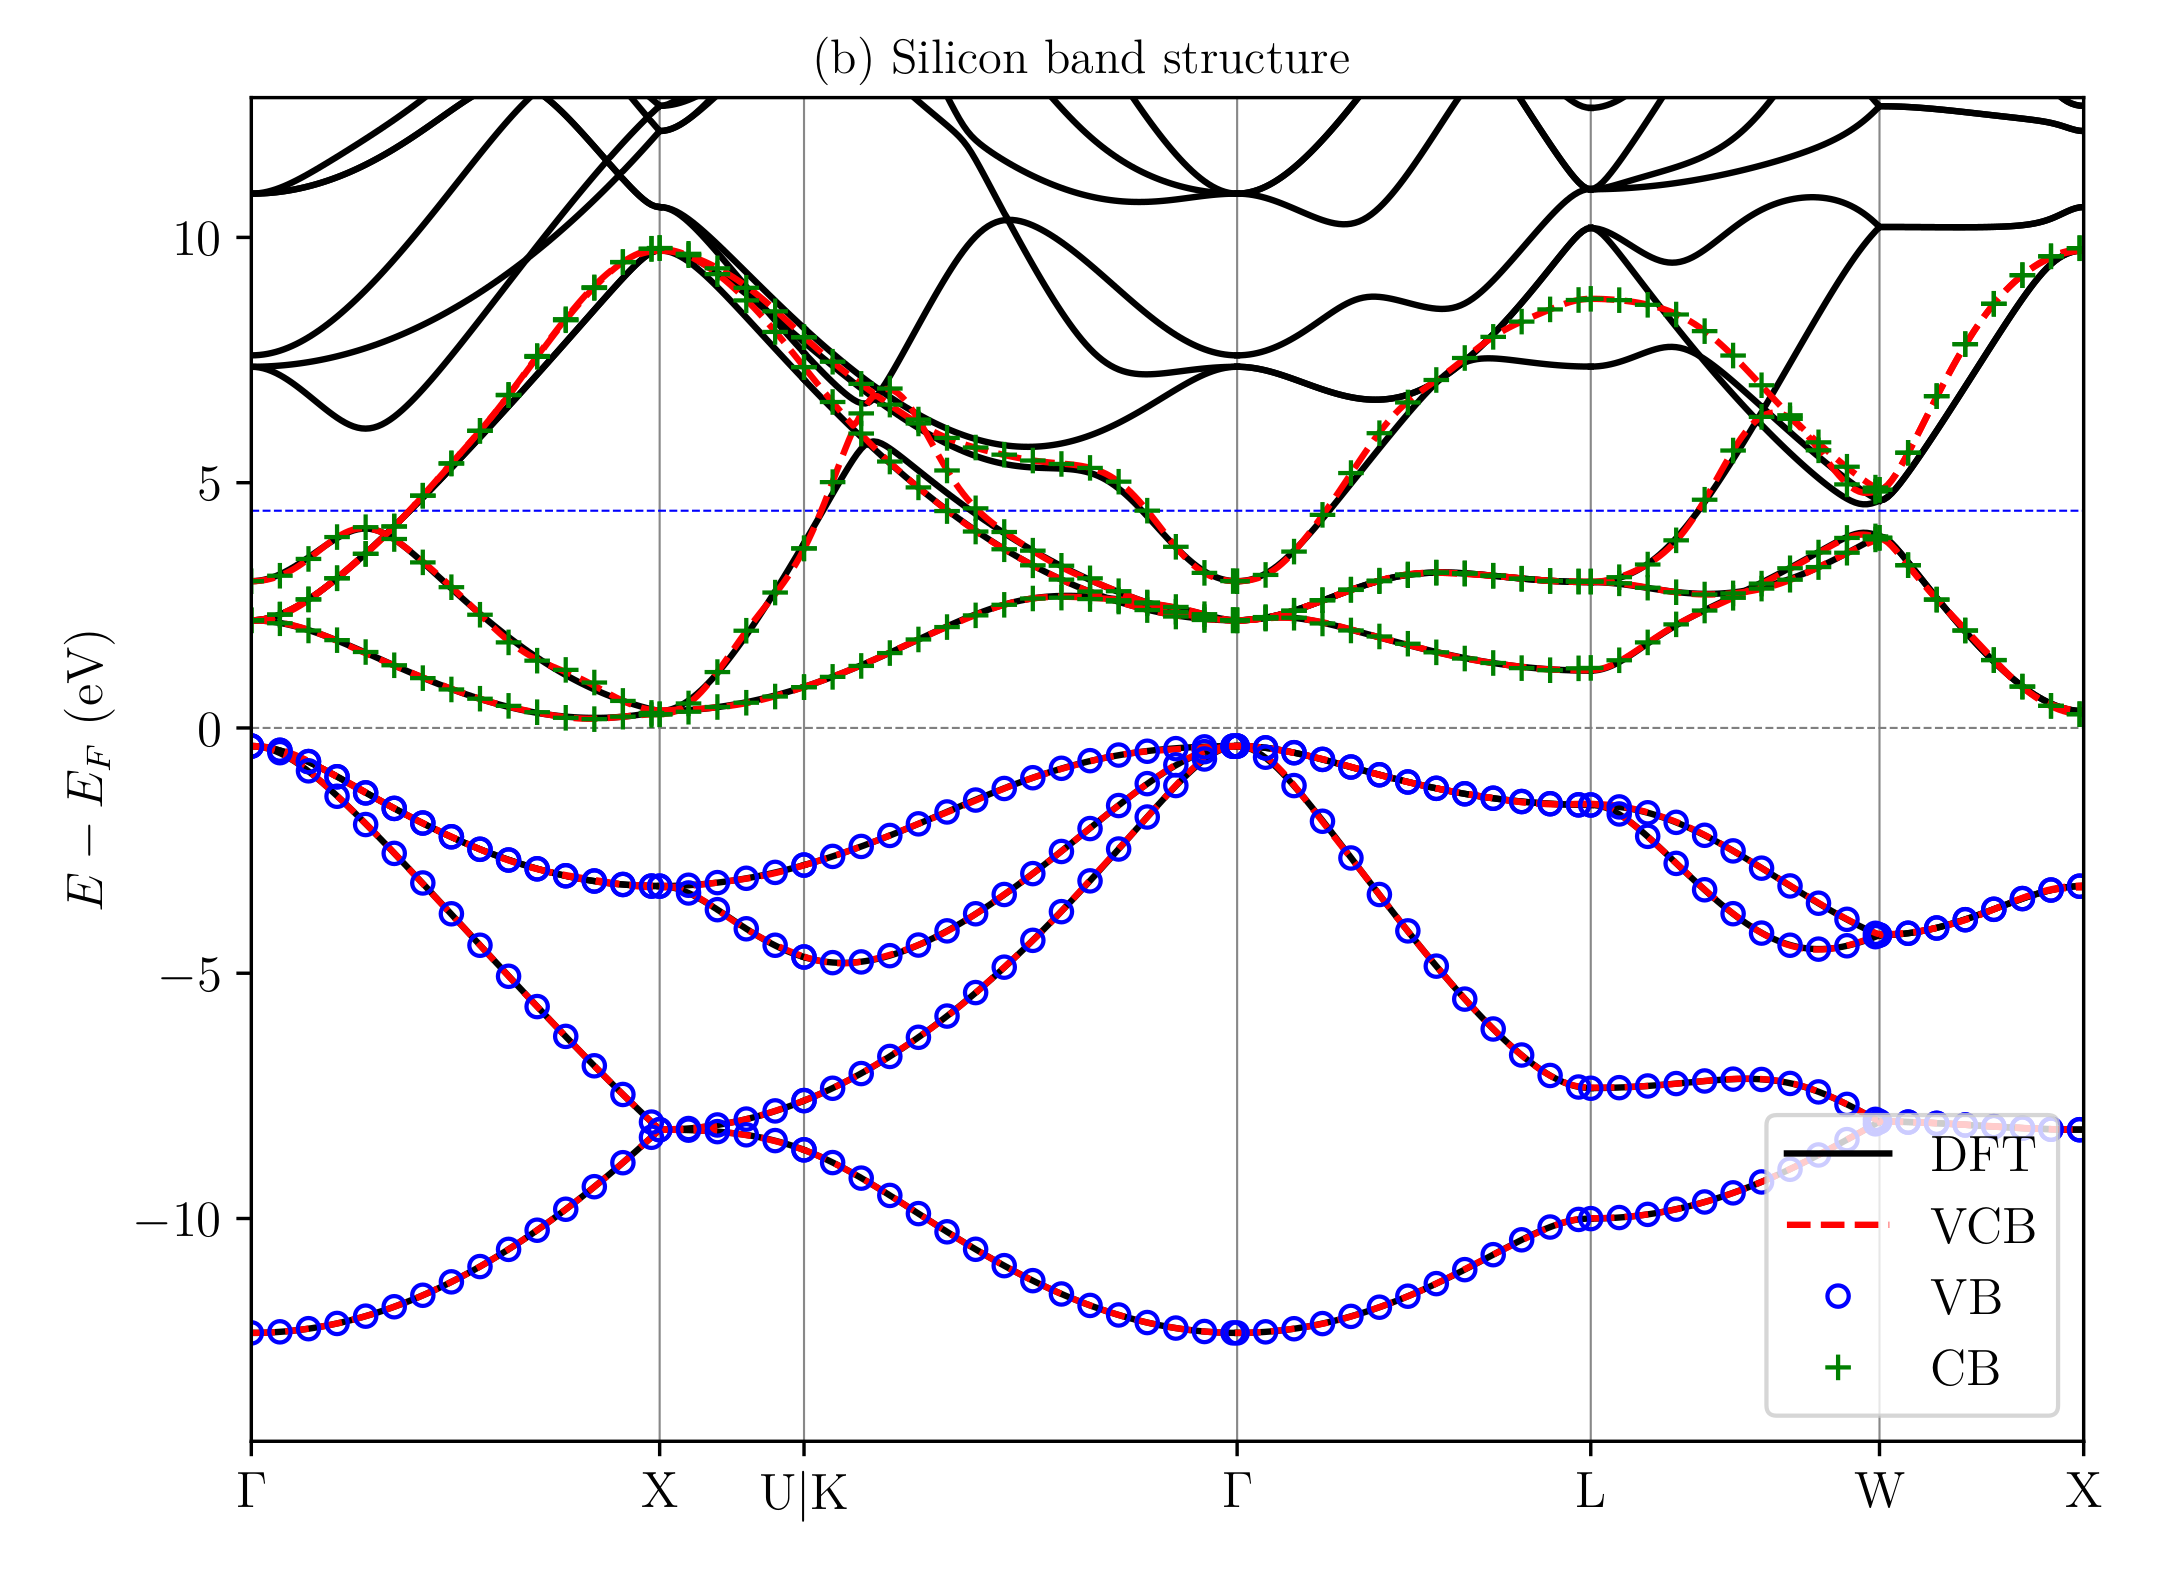
\includegraphics[width=0.5\columnwidth]{figures/target_manifolds_fig1b.png}
         }
      \end{figure}

   \blfootcite{Qiao2023a}
\end{frame}


\begin{frame}{Recent improvements: screening via DFPT}
   Original formulation requires explicit charged defect calculations in a supercell

   \begin{equation*}
   \alpha^{n+1}_i =
   \alpha^n_i \frac{\Delta E^\text{Koopmans}_i - \lambda_{ii}(0, 1)}{\lambda_{ii}(\alpha^n_i, 1) - \lambda_{ii}(0, 1)}; \qquad  \Delta E^\text{Koopmans}_i = E^\text{Koopmans}(N) - E^\text{Koopmans}_i(N - 1)
   \end{equation*}

   \onslide<2->{
   Now reformulated in terms of DFPT\footcite{Colonna2019}...

   \begin{equation*}
   \alpha_{i} = 1 + \frac{\langle v^{i}_\mathsf{pert} \vert \Delta^{i} n \rangle}{\langle n_{i} \vert v^{i}_\mathsf{pert} \rangle}.
   \end{equation*}
   }
   
   \onslide<3->{
   ... in reciprocal space\footcite{Colonna2022}
   \begin{equation*}
      \alpha_{\mathbf{0}i} =  1 + \frac{\sum_{\mathbf{q}} \langle v^{\mathbf{0}i}_\mathsf{pert,\mathbf{q}} \vert \Delta^{\mathbf{0}i}_{\mathbf{q}}n \rangle} {\sum_{\mathbf{q}} \langle n^{\mathbf{0}i}_{\mathbf{q}} \vert v^{\mathbf{0}i}_\mathsf{pert,\mathbf{q}} \rangle}.
   \end{equation*}
   }

\end{frame}

\begin{frame}{Recent improvements: spin-orbit coupling}
   \centering
   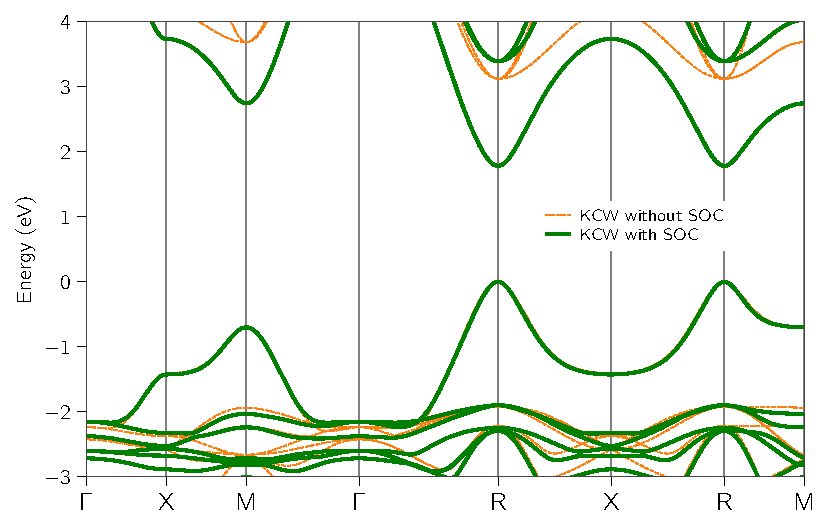
\includegraphics[width=0.5\textwidth]{figures/marrazzo_CsPbBr3_bands.pdf}

   \begin{tabular}{c S[table-format = 2.2] S[table-format = 2.2] S[table-format = 2.2] >{\color{seaborn_red}\bfseries}S[table-format = 2.2] S[table-format = 2.2] S[table-format = 2.2]}
      CsPbBr\textsubscript{3}
                       & {LDA} & {HSE} & {G\textsubscript{0}W\textsubscript{0}} & {KI} & {QSG$\tilde{\mathsf{W}}$} & {exp} \\
      \midrule
      without SOC & 1.40  & 2.09 & 2.56 & 3.12 & 3.15 & {\multirow{2}{*}{1.85}} \\
      with SOC         & 0.18 & 0.78 & 0.94 & 1.78 & 1.53      %                                  & {MAPE (\%)} & 15.58 & 5.71                                   & 2.99 & 3.14   & 7.41
   \end{tabular}
   \blfootcite{Marrazzo2024}

\end{frame}

\begin{frame}{Recent improvements: automated workflows}
   \small We have complicated workflows, with either...

   \vspace{1ex}

   \onslide<2->{
      (a) finite difference calculations using a supercell

      \vspace{-2ex}
      \adjustbox{width=\textwidth}{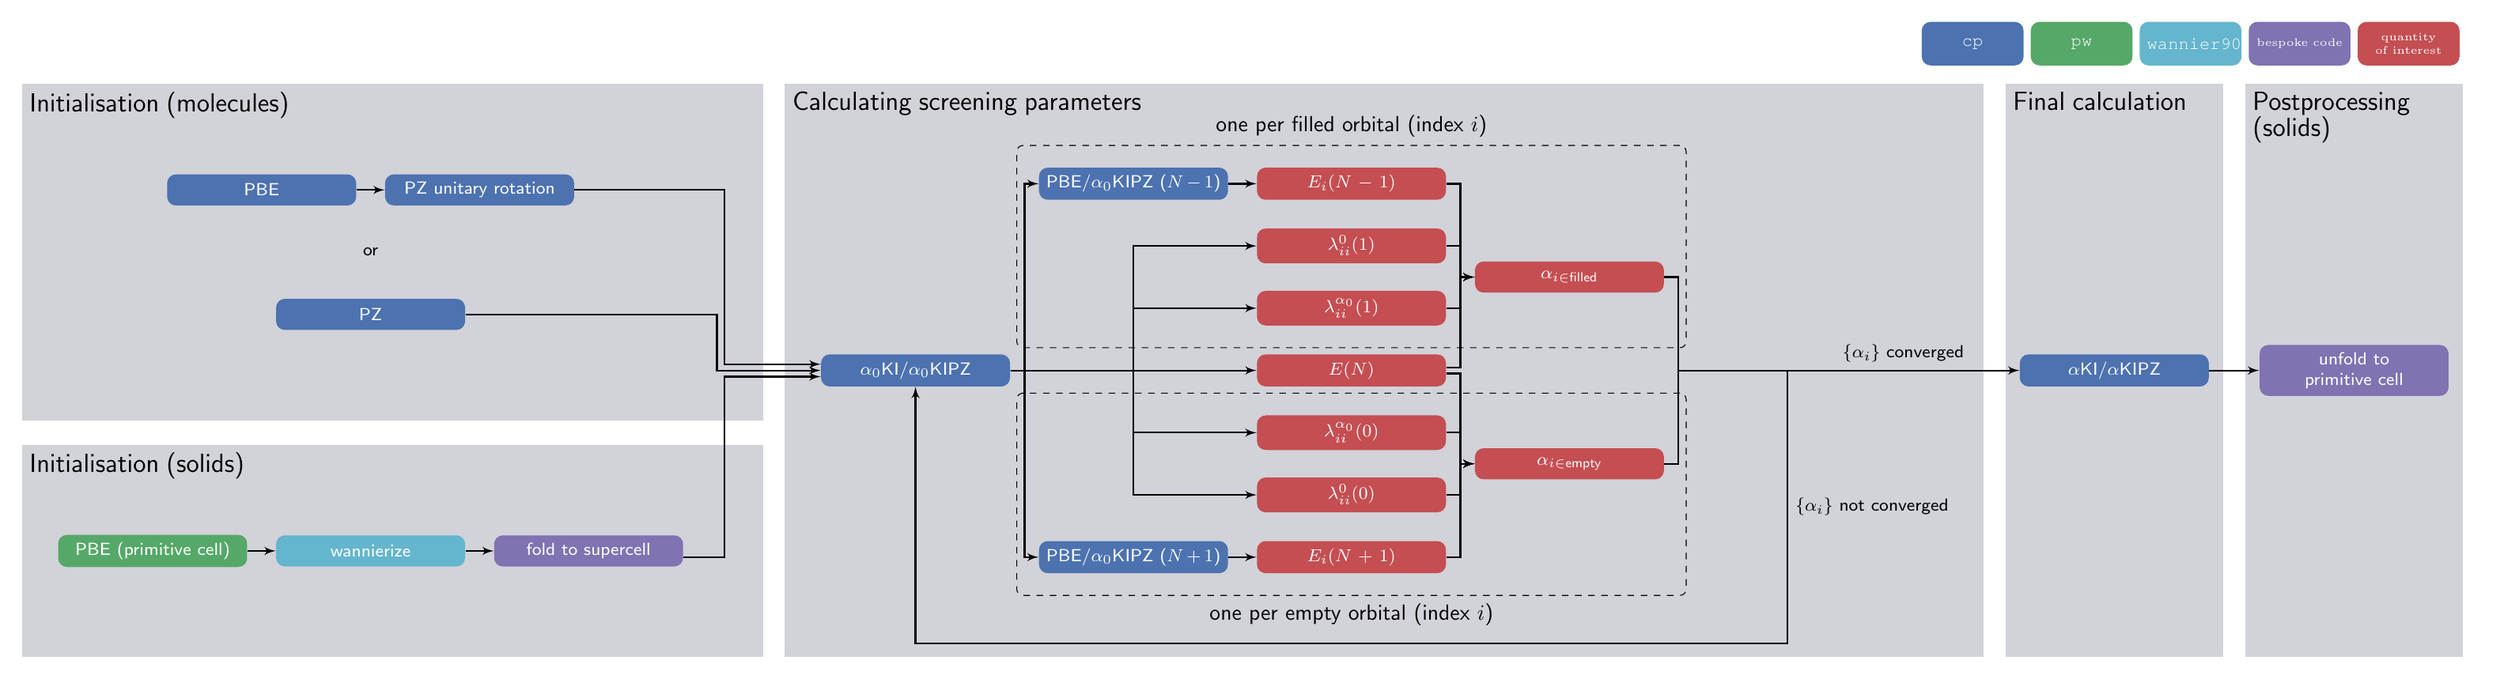
\begin{tikzpicture}[font=\tiny, x=3.5cm, y=1cm]
\begin{pgfonlayer}{background}
   % \node[fit= (KC init) (empty label) (filled label) (sc loop 1) (converged label), fill=seaborn_bg_grey, inner sep=0.5cm] (calculating screening) {};
   % \node [dummy, above=0cm of calculating screening, font=\sffamily]{Calculating screening parameters};
   \fill [seaborn_bg_grey_dark] (-2.1,-0.8) rectangle (1.3,4.6);
   \node at (-2.1, 4.6) [default_text] {\large Initialisation (molecules)};
   \fill [seaborn_bg_grey_dark] (-2.1,-4.6) rectangle (1.3,-1.2);
   \node at (-2.1, -1.2) [default_text] {\large Initialisation (solids)};
   \fill [seaborn_bg_grey_dark] (1.4,-4.6) rectangle (6.9,4.6);
   \node at (1.4, 4.6) [default_text] {\large Calculating screening parameters};
   \fill [seaborn_bg_grey_dark] (7,-4.6) rectangle (8,4.6);
   \node at (7, 4.6) [default_text, text width=3.5cm] {\large Final calculation};
   \fill [seaborn_bg_grey_dark] (8.1,-4.6) rectangle (9.1,4.6);
   \node at (8.1, 4.6) [default_text, text width=3.5cm] {\large Postprocessing (solids)};
\end{pgfonlayer}

% Key
\node at (6.85, 5.25) [cp, text width=1.4cm, minimum height=0.7cm] {\texttt{cp}};
\node at (7.35, 5.25) [pw, text width=1.4cm, minimum height=0.7cm] {\texttt{pw}};
\node at (7.85, 5.25) [wannier90, text width=1.4cm, minimum height=0.7cm] {\texttt{wannier90}};
\node at (8.35, 5.25) [bespoke, text width=1.4cm, minimum height=0.7cm, font=\tiny] {bespoke code};
\node at (8.85, 5.25) [observable, text width=1.4cm, minimum height=0.7cm, font=\tiny] {quantity of interest};

% Initialisation
% Option 1
\node at (-1, 2.9) [cp] (PBE init) {PBE};
\node at (0, 2.9) [cp] (PZ innerloop) {PZ unitary rotation};
\path [line] (PBE init) -- (PZ innerloop);

% OR
\node at (-0.5, 1.9) [default] (or) {or};

% Option 2
\node at (-0.5, 0.9) [cp] (PZ init) {PZ};

% Solids
\node at (-1.5, -2.9) [pw] (pw PBE init) {PBE (primitive cell)};
\node at (-0.5, -2.9) [wannier90] (wannierize) {wannierize};
\node at (0.5, -2.9) [bespoke] (unfold) {fold to supercell};
\path [line] (pw PBE init) -- (wannierize);
\path [line] (wannierize) -- (unfold);

% Calculating screening parameters
\node at (2, 0) [cp] (KC init) {$\alpha_0$KI/$\alpha_0$KIPZ};

\path let
\p1 = (PZ innerloop),
\p2 = (unfold.east)
in
coordinate (dummy) at (\x2, \y1);
\path let
\p1 = (PZ init),
\p2 = (unfold.east)
in
coordinate (dummy2) at (\x2, \y1);
\path [line] (PZ innerloop) -- (dummy) to[-|-=0.3] ([yshift=2\myyshift]KC init.west);
\path [line] (PZ init.east) -- ([xshift=-3.5\myyshift]dummy2) to[-|-=0.3] (KC init.west);
\path [line] ([yshift=-2\myyshift]unfold.east) to[-|-=0.3] ([yshift=-2\myyshift]KC init.west);

% KI filled %%%%%%%%%%%%%%%%%%%%%%%%%%%%%%%%%%%%%%%%%%%%%%%%%%

% calculations
\node at (3, 3) [cp] (N-1_filled) {PBE/$\alpha_0$KIPZ ($N-1$)};
\node at (3, -3) [cp] (N+1_empty) {PBE/$\alpha_0$KIPZ ($N+1$)};

\path [line] (KC init) to[-|-] (N-1_filled);
\path [line] (KC init) to[-|-] (N+1_empty);

% results
\node at (4, 3) [observable] (EN-1_filled) {$E_i(N-1)$};
\node at (4, 2) [observable] (lambda0_filled) {$\lambda^{0}_{ii}(1)$};
\node at (4, 1) [observable] (lambda_filled) {$\lambda^{\alpha_0}_{ii}(1)$};
\node at (4, 0) [observable] (EN) {$E(N)$};
\node at (4, -1) [observable] (lambda_empty) {$\lambda^{\alpha_0}_{ii}(0)$};
\node at (4, -2) [observable] (lambda0_empty) {$\lambda^{0}_{ii}(0)$};
\node at (4, -3) [observable] (EN+1_empty) {$E_i(N+1)$};

\path [line] (KC init) -- (EN);
\path [line] (KC init.east) to[-|-] (lambda_filled.west);
\path [line] (KC init.east) to[-|-] (lambda_empty.west);
\path [line] (KC init.east) to[-|-] (lambda0_filled.west);
\path [line] (KC init.east) to[-|-] (lambda0_empty.west);

\path [line] (N-1_filled) -- (EN-1_filled);

\path [line] (N+1_empty) -- (EN+1_empty);

% alpha parameters
\node at (5, 1.5) [observable] (alpha filled) {$\alpha_{i \in \text{filled}}$};
\node at (5, -1.5) [observable] (alpha empty) {$\alpha_{i \in \text{empty}}$};

\path [line] (lambda_filled) to[-|-] (alpha filled);
\path [line] ([yshift=\myyshift]EN.east) to[-|-] (alpha filled.west);
\path [line] (lambda0_filled) to[-|-] (alpha filled);
\path [line] (EN-1_filled) to[-|-] (alpha filled);

\path [line] (lambda_empty) to[-|-] (alpha empty);
\path [line] ([yshift=-\myyshift]EN.east) to[-|-] (alpha empty.west);
\path [line] (lambda0_empty) to[-|-] (alpha empty);
\path [line] (EN+1_empty) to[-|-] (alpha empty);

% SC check
\coordinate (sc check) at (6, 0);
\path [headless_line] (alpha empty) to[-|-] (sc check);
\path [headless_line] (alpha filled) to[-|-] (sc check);

% SC loop
\node [below= of EN+1_empty] (sc loop y) {};
\path let
\p1 = (sc check),
\p2 = (sc loop y)
in
coordinate (sc loop 1) at (\x1, \y2);
\path [line] (sc check) -- node [midway, right, font=\sffamily] (not converged label) {\footnotesize $\{\alpha_i\}$ not converged} (sc loop 1) -| (KC init.south);

% Final calc
\node at (7.5, 0) [cp] (final KI) {$\alpha$KI/$\alpha$KIPZ};
\path [line] (sc check) -- node [midway, above, font=\sffamily] (converged label) {\footnotesize $\{\alpha_i\}$ converged} (final KI);

% Postproc
\node at (8.6, 0) [bespoke] (upfold) {unfold to primitive cell};
\path [line] (final KI) -- (upfold);

% Boxes
% Screening parametere
\node [boxwhite, fit= (N-1_filled) (lambda_filled) (alpha filled),
   draw, dashed, fill opacity=0, inner sep=0.35cm](filled box){};
\node [dummy, above=0cm of filled box, font=\sffamily](filled label){one per filled orbital (index $i$)};
\node [boxwhite, fit= (N+1_empty) (lambda_empty) (alpha empty),
   draw, dashed, fill opacity=0, inner sep=0.35cm](empty box){};
\node [dummy, below=0cm of empty box, font=\sffamily](empty label){one per empty orbital (index $i$)};

% \onslide<2->{
%    \node at (3.5, 0) [default_text, fill=white, opacity=0.9, text opacity=1, anchor=center, minimum height=5cm, text width=7.5cm, execute at begin node=\setlength{\baselineskip}{30pt}] (nc text) {
%       \huge Riccardo De Gennaro
%       \textbf{M22.00004} / paper in preparation
%    };
%    \node[right = -0.2cm of nc text, anchor=west]{\includegraphics[height=5cm]{figures/riccardo_degennaro.jpg}};
% }


% ML
\end{tikzpicture}}
   }

   \vspace{-1.5ex}
   \onslide<3->{
      (b) DFPT using a primitive cell

      \vspace{-2ex}
      \adjustbox{width=0.655\textwidth}{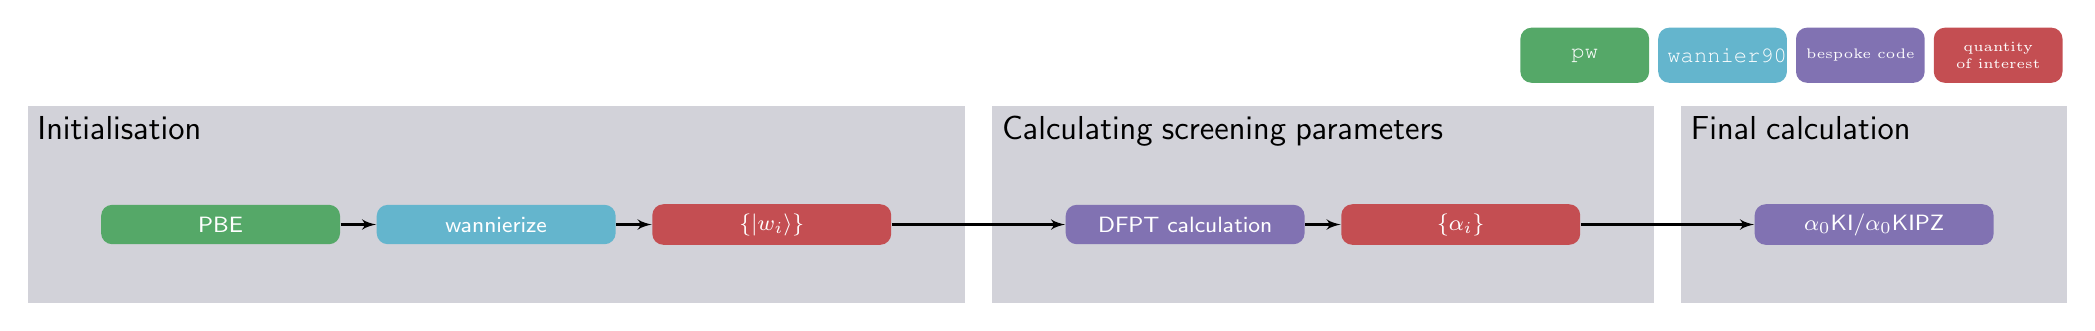
\begin{tikzpicture}[font=\tiny, x=3.5cm, y=1cm]
   \begin{pgfonlayer}{background}
      \fill [seaborn_bg_grey_dark] (-2.2,-1) rectangle (1.2,1.5);
      \node at (-2.2, 1.5) [default_text] {\large Initialisation};
      \fill [seaborn_bg_grey_dark] (1.3,-1) rectangle (3.7,1.5);
      \node at (1.3, 1.5) [default_text] {\large Calculating screening parameters};
      \fill [seaborn_bg_grey_dark] (3.8,-1) rectangle (5.2,1.5);
      \node at (3.8, 1.5) [default_text, text width=3.5cm] {\large Final calculation};
      % \fill [seaborn_bg_grey_dark] (8.1,-1) rectangle (9.1,1.5);
      % \node at (8.1, 1.5) [default_text, text width=3.5cm] {\large Postprocessing};
   \end{pgfonlayer}

   % Key
   \node at (3.45, 2.15) [pw, text width=1.4cm, minimum height=0.7cm] {\texttt{pw}};
   \node at (3.95, 2.15) [wannier90, text width=1.4cm, minimum height=0.7cm] {\texttt{wannier90}};
   \node at (4.45, 2.15) [bespoke, text width=1.4cm, minimum height=0.7cm, font=\tiny] {bespoke code};
   \node at (4.95, 2.15) [observable, text width=1.4cm, minimum height=0.7cm, font=\tiny] {quantity of interest};

   % Initialisation
   % Solids
   \node at (-1.5, 0) [pw] (pw PBE init) {PBE};
   \node at (-0.5, 0) [wannier90] (wannierize) {wannierize};
   \node at (0.5, 0) [observable] (unfold) {$\{\ket{w_i}\}$};
   \path [line] (pw PBE init) -- (wannierize);
   \path [line] (wannierize) -- (unfold);

   % Calculating screening parameters
   \node at (2, 0) [bespoke] (KC screen) {DFPT calculation};
   \node at (3, 0) [observable] (alphas) {$\{\alpha_i\}$};
   \path [line] (unfold) -- (KC screen);
   \path [line] (KC screen) -- (alphas);

   % Final calc
   \node at (4.5, 0) [bespoke] (KC ham) {$\alpha_0$KI/$\alpha_0$KIPZ};
   \path [line] (alphas) -- (KC ham);

   % \onslide<4->{
   %    \node at (1, 0) [default_text, fill=white, opacity=0.9, text opacity=1, anchor=center, minimum height=5cm, text width=7cm, execute at begin node=\setlength{\baselineskip}{30pt}] (nc text) {
   %       \huge Nicola Colonna
   %       \textbf{A20.00002} /
   %       paper in preparation
   %    };
   %    \node[right = -0.2cm of nc text, anchor=west]{\includegraphics[height=5cm]{figures/nicola_colonna.png}};
   % }
    % \onslide<4->{
    %   \fill [seaborn_bg_grey_dark,opacity=0.8] (1.3,-1) rectangle (3.7,1.5);
    %   \node at (2.5, 0) [cp, fill=seaborn_yellow, font=\Huge, inner sep=10pt] (ml) {ML model};
    %   \path [headless_line] (unfold) -- (ml);
    %   \path [line] (ml) -- (KC ham);
    % }
\end{tikzpicture}
}
   }

   \blfootcite{Linscott2023}
   % \onslide<6>{
   %    \vspace{-0.375\paperheight}
   %    \begin{flushright}
   %       \begin{tcolorbox}[enhanced jigsaw, width=4cm, opacityback=0, colframe=seaborn_red, coltext=seaborn_red, left=3pt, bottom=3pt, top=3pt, right=3pt, tikz={rotate=30,transform shape}, boxrule=1.5mm]
   %          \begin{center}
   %             \includegraphics[height=1cm]{./figures/qe_logo_high_res_cropped.jpg}
   %             \bf \huge\ \raisebox{0.3cm}{+}\,
   %             \includegraphics[height=1cm]{./figures/python_logo.png}

   %             \bf \large OUT NOW!
   %          \end{center}
   %       \end{tcolorbox}
   %    \end{flushright}
   % }

\end{frame}


% \begin{frame}{Recent improvements: automated workflows}
% 
%    % \texttt{kcw.x} (DFPT implementation) is distributed in Quantum ESPRESSO v7.1 onwards
% 
%    % \vspace{4ex}
% 
%    Complicated workflows mean that...
%    \begin{itemize}
%       \item lots of different codes that need to handshake
%       \item lots of scope for human error
%       \item reproducibility becomes difficult
%       \item expert knowledge required
%    \end{itemize}
% 
%    Our solution...
% 
% \end{frame}

\begin{frame}{}
   \vspace{-1ex}
   \begin{center}
      
\includegraphics[width=0.6\textwidth]{figures/koopmans_grey_on_transparent.png}
   \end{center}

   \vspace{-2ex}

   \begin{columns}
      \begin{column}{0.55\textwidth}
         \begin{itemize}
            \item v1.0 released last year\footnotemark[1]
            \item implementations of Koopmans functionals within Quantum ESPRESSO
            \item automated workflows
                  \begin{itemize}
                     \item start-to-finish Koopmans calculations
                     \item Wannierization
                     \item dielectric tensor
                     \item convergence tests
                     \item ...
                  \end{itemize}
            \item built on top of ASE\footnotemark[2]
            \item does not require expert knowledge
         \end{itemize}
      \end{column}

      \begin{column}{0.4\textwidth}
         \centering
         \url{koopmans-functionals.org}
         
\includegraphics[width=\columnwidth]{figures/website_cropped.png}
      \end{column}
   \end{columns}
   \footnotetext[1]{\cite{Linscott2023}}
   \footnotetext[2]{\cite{Larsen2017}}
\end{frame}

% \begin{frame}{Neutral excitations with Koopmans}
%    \centering
%    \includegraphics[width=0.5\textwidth]{figures/elliott_workflow.jpeg}
%    \blfootcite{Elliott2019}
% \end{frame}
% 
% \begin{frame}{Neutral excitations with Koopmans}
%    \begin{columns}
%       \begin{column}{0.4\textwidth}
%          \includegraphics[width=\textwidth]{figures/elliott_scatter2.jpeg}
%       \end{column}
%       \begin{column}{0.6\textwidth}
%          \footnotesize
%          \begin{tabular}{c >{\color{seaborn_red}\bfseries}S[table-format = 2.2] S[table-format = 2.2] S[table-format = 2.2] S[table-format = 2.2] S[table-format = 2.2]}
%             \multirow{2}{*}{Thiel's set} & {KI-BSE} & \multicolumn{2}{c}{G$_0$W$_0$-BSE} & \multicolumn{2}{c}{TDDFT}                   \\
%                                          & {PBE}    & {PBE}                              & {B3LYP}                   & {PBE} & {B3LYP} \\
%             \hline
%             MAE (eV)                     & 0.54     & 0.83                               & 0.46                      & 0.55  & 0.27
%          \end{tabular}
% 
%          \vspace{2ex}
%          \onslide<2->{
%             Based on RPA $\rightarrow$ room for improvement with finite-field approaches
%          }
% 
%       \end{column}
%    \end{columns}
%    \centering
% 
%    \vspace{1ex}
%    \blfootcite{Elliott2019}
%    \blfootcite{Nguyen2019}
% 
% \end{frame}
\begin{frame}{koopmans: the input file}
   \begin{minipage}[t]{0.475\columnwidth}
      \inputminted[fontsize=\tiny,breaklines,lastline=20]{json}{scripts/si_auto_wann.json}
   \end{minipage}
   \hspace{0.025\textwidth}
   \begin{minipage}[t]{0.475\columnwidth}
      \inputminted[fontsize=\tiny,breaklines,firstline=21]{json}{scripts/si_auto_wann.json}
   \end{minipage}
\end{frame}

% \begin{frame}{koopmans: the output file}
%    \vspace{-2ex}
%    \only<1>{
%       \inputminted[fontsize=\scriptsize,breaklines]{text}{scripts/si_ki_full.out}
%    }
%    \only<2>{
%       \inputminted[fontsize=\scriptsize,breaklines,firstline=25]{text}{scripts/si_ki_full.out}
%    }
%    \only<3>{
%       \inputminted[fontsize=\scriptsize,breaklines,firstline=50]{text}{scripts/si_ki_full.out}
%    }
%    \only<4>{
%       \inputminted[fontsize=\scriptsize,breaklines,firstline=75]{text}{scripts/si_ki_full.out}
%    }
% \end{frame}

\begin{frame}{koopmans is scriptable}
   \vspace{-2ex}
   \inputminted[fontsize=\scriptsize,breaklines]{python}{scripts/si_auto_wann.py}
\end{frame}



\begin{frame}{Take home messages}

   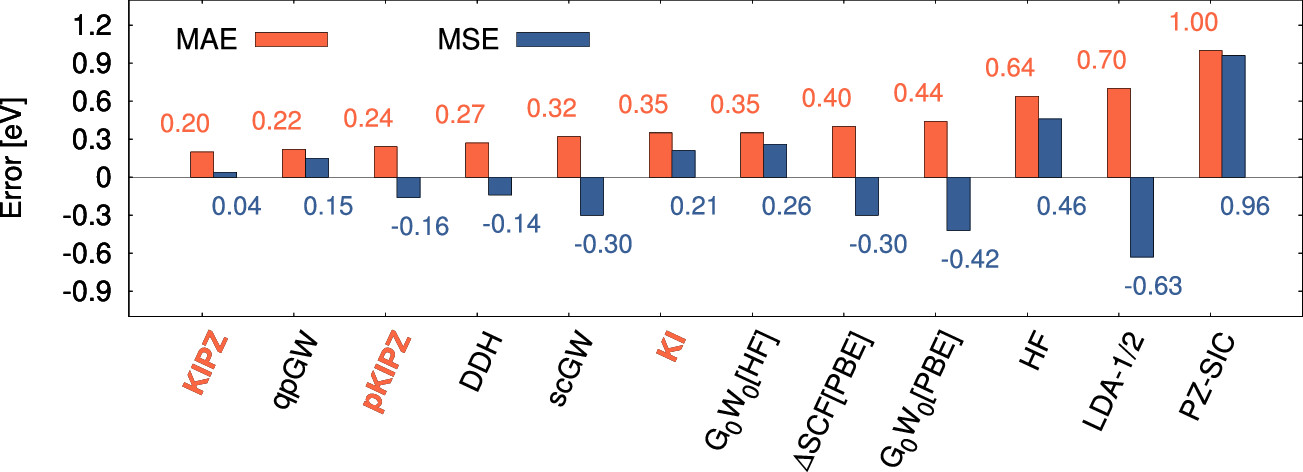
\includegraphics[height=0.2\paperheight]{figures/colonna_2019_gw100_ip.jpeg}
   \hfill
   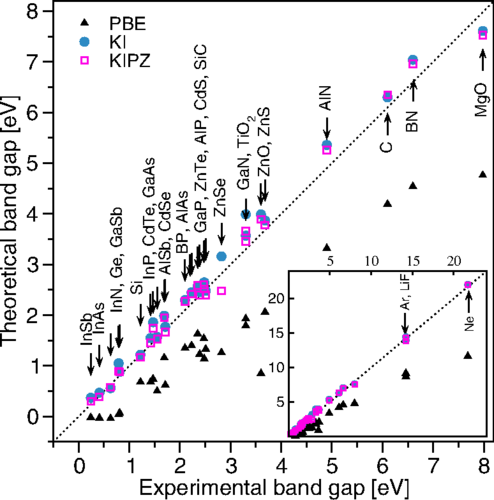
\includegraphics[height=0.2\paperheight]{figures/fig_nguyen_prx_bandgaps.png}
   \hfill
   \adjustbox{height=0.2\paperheight}{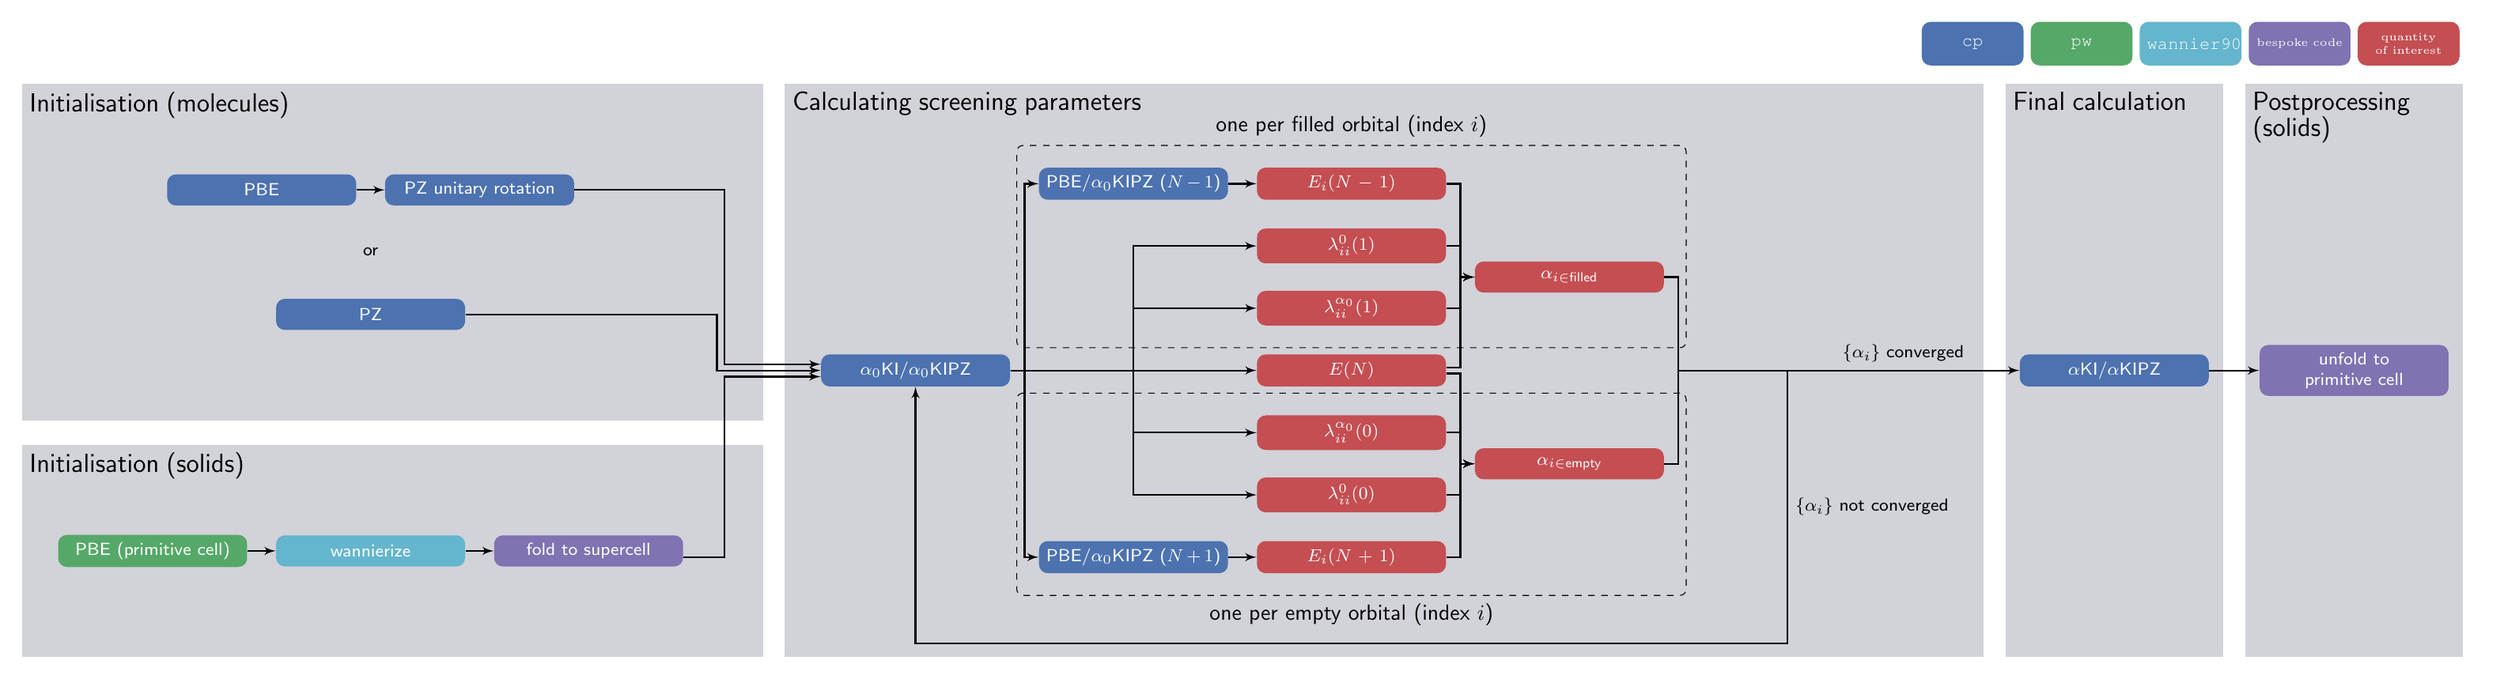
\begin{tikzpicture}[font=\tiny, x=3.5cm, y=1cm]
\begin{pgfonlayer}{background}
   % \node[fit= (KC init) (empty label) (filled label) (sc loop 1) (converged label), fill=seaborn_bg_grey, inner sep=0.5cm] (calculating screening) {};
   % \node [dummy, above=0cm of calculating screening, font=\sffamily]{Calculating screening parameters};
   \fill [seaborn_bg_grey_dark] (-2.1,-0.8) rectangle (1.3,4.6);
   \node at (-2.1, 4.6) [default_text] {\large Initialisation (molecules)};
   \fill [seaborn_bg_grey_dark] (-2.1,-4.6) rectangle (1.3,-1.2);
   \node at (-2.1, -1.2) [default_text] {\large Initialisation (solids)};
   \fill [seaborn_bg_grey_dark] (1.4,-4.6) rectangle (6.9,4.6);
   \node at (1.4, 4.6) [default_text] {\large Calculating screening parameters};
   \fill [seaborn_bg_grey_dark] (7,-4.6) rectangle (8,4.6);
   \node at (7, 4.6) [default_text, text width=3.5cm] {\large Final calculation};
   \fill [seaborn_bg_grey_dark] (8.1,-4.6) rectangle (9.1,4.6);
   \node at (8.1, 4.6) [default_text, text width=3.5cm] {\large Postprocessing (solids)};
\end{pgfonlayer}

% Key
\node at (6.85, 5.25) [cp, text width=1.4cm, minimum height=0.7cm] {\texttt{cp}};
\node at (7.35, 5.25) [pw, text width=1.4cm, minimum height=0.7cm] {\texttt{pw}};
\node at (7.85, 5.25) [wannier90, text width=1.4cm, minimum height=0.7cm] {\texttt{wannier90}};
\node at (8.35, 5.25) [bespoke, text width=1.4cm, minimum height=0.7cm, font=\tiny] {bespoke code};
\node at (8.85, 5.25) [observable, text width=1.4cm, minimum height=0.7cm, font=\tiny] {quantity of interest};

% Initialisation
% Option 1
\node at (-1, 2.9) [cp] (PBE init) {PBE};
\node at (0, 2.9) [cp] (PZ innerloop) {PZ unitary rotation};
\path [line] (PBE init) -- (PZ innerloop);

% OR
\node at (-0.5, 1.9) [default] (or) {or};

% Option 2
\node at (-0.5, 0.9) [cp] (PZ init) {PZ};

% Solids
\node at (-1.5, -2.9) [pw] (pw PBE init) {PBE (primitive cell)};
\node at (-0.5, -2.9) [wannier90] (wannierize) {wannierize};
\node at (0.5, -2.9) [bespoke] (unfold) {fold to supercell};
\path [line] (pw PBE init) -- (wannierize);
\path [line] (wannierize) -- (unfold);

% Calculating screening parameters
\node at (2, 0) [cp] (KC init) {$\alpha_0$KI/$\alpha_0$KIPZ};

\path let
\p1 = (PZ innerloop),
\p2 = (unfold.east)
in
coordinate (dummy) at (\x2, \y1);
\path let
\p1 = (PZ init),
\p2 = (unfold.east)
in
coordinate (dummy2) at (\x2, \y1);
\path [line] (PZ innerloop) -- (dummy) to[-|-=0.3] ([yshift=2\myyshift]KC init.west);
\path [line] (PZ init.east) -- ([xshift=-3.5\myyshift]dummy2) to[-|-=0.3] (KC init.west);
\path [line] ([yshift=-2\myyshift]unfold.east) to[-|-=0.3] ([yshift=-2\myyshift]KC init.west);

% KI filled %%%%%%%%%%%%%%%%%%%%%%%%%%%%%%%%%%%%%%%%%%%%%%%%%%

% calculations
\node at (3, 3) [cp] (N-1_filled) {PBE/$\alpha_0$KIPZ ($N-1$)};
\node at (3, -3) [cp] (N+1_empty) {PBE/$\alpha_0$KIPZ ($N+1$)};

\path [line] (KC init) to[-|-] (N-1_filled);
\path [line] (KC init) to[-|-] (N+1_empty);

% results
\node at (4, 3) [observable] (EN-1_filled) {$E_i(N-1)$};
\node at (4, 2) [observable] (lambda0_filled) {$\lambda^{0}_{ii}(1)$};
\node at (4, 1) [observable] (lambda_filled) {$\lambda^{\alpha_0}_{ii}(1)$};
\node at (4, 0) [observable] (EN) {$E(N)$};
\node at (4, -1) [observable] (lambda_empty) {$\lambda^{\alpha_0}_{ii}(0)$};
\node at (4, -2) [observable] (lambda0_empty) {$\lambda^{0}_{ii}(0)$};
\node at (4, -3) [observable] (EN+1_empty) {$E_i(N+1)$};

\path [line] (KC init) -- (EN);
\path [line] (KC init.east) to[-|-] (lambda_filled.west);
\path [line] (KC init.east) to[-|-] (lambda_empty.west);
\path [line] (KC init.east) to[-|-] (lambda0_filled.west);
\path [line] (KC init.east) to[-|-] (lambda0_empty.west);

\path [line] (N-1_filled) -- (EN-1_filled);

\path [line] (N+1_empty) -- (EN+1_empty);

% alpha parameters
\node at (5, 1.5) [observable] (alpha filled) {$\alpha_{i \in \text{filled}}$};
\node at (5, -1.5) [observable] (alpha empty) {$\alpha_{i \in \text{empty}}$};

\path [line] (lambda_filled) to[-|-] (alpha filled);
\path [line] ([yshift=\myyshift]EN.east) to[-|-] (alpha filled.west);
\path [line] (lambda0_filled) to[-|-] (alpha filled);
\path [line] (EN-1_filled) to[-|-] (alpha filled);

\path [line] (lambda_empty) to[-|-] (alpha empty);
\path [line] ([yshift=-\myyshift]EN.east) to[-|-] (alpha empty.west);
\path [line] (lambda0_empty) to[-|-] (alpha empty);
\path [line] (EN+1_empty) to[-|-] (alpha empty);

% SC check
\coordinate (sc check) at (6, 0);
\path [headless_line] (alpha empty) to[-|-] (sc check);
\path [headless_line] (alpha filled) to[-|-] (sc check);

% SC loop
\node [below= of EN+1_empty] (sc loop y) {};
\path let
\p1 = (sc check),
\p2 = (sc loop y)
in
coordinate (sc loop 1) at (\x1, \y2);
\path [line] (sc check) -- node [midway, right, font=\sffamily] (not converged label) {\footnotesize $\{\alpha_i\}$ not converged} (sc loop 1) -| (KC init.south);

% Final calc
\node at (7.5, 0) [cp] (final KI) {$\alpha$KI/$\alpha$KIPZ};
\path [line] (sc check) -- node [midway, above, font=\sffamily] (converged label) {\footnotesize $\{\alpha_i\}$ converged} (final KI);

% Postproc
\node at (8.6, 0) [bespoke] (upfold) {unfold to primitive cell};
\path [line] (final KI) -- (upfold);

% Boxes
% Screening parametere
\node [boxwhite, fit= (N-1_filled) (lambda_filled) (alpha filled),
   draw, dashed, fill opacity=0, inner sep=0.35cm](filled box){};
\node [dummy, above=0cm of filled box, font=\sffamily](filled label){one per filled orbital (index $i$)};
\node [boxwhite, fit= (N+1_empty) (lambda_empty) (alpha empty),
   draw, dashed, fill opacity=0, inner sep=0.35cm](empty box){};
\node [dummy, below=0cm of empty box, font=\sffamily](empty label){one per empty orbital (index $i$)};

% \onslide<2->{
%    \node at (3.5, 0) [default_text, fill=white, opacity=0.9, text opacity=1, anchor=center, minimum height=5cm, text width=7.5cm, execute at begin node=\setlength{\baselineskip}{30pt}] (nc text) {
%       \huge Riccardo De Gennaro
%       \textbf{M22.00004} / paper in preparation
%    };
%    \node[right = -0.2cm of nc text, anchor=west]{\includegraphics[height=5cm]{figures/riccardo_degennaro.jpg}};
% }


% ML
\end{tikzpicture}}

   \begin{itemize}
      \item Koopmans functionals are a class of functionals that treat spectral properties on the same footing as total energy differences (via GPWL)
      \item they can give orbital energies and band structures with comparable accuracy to state-of-the-art GW
      \item the \texttt{koopmans} package simplifies running these calculations
   \end{itemize}

\end{frame}

% \begin{frame}{Take home messages}
%    \includegraphics[width=\textwidth]{figures/jctc.png}
% \end{frame}

% Acknowledgements
\begingroup
\setbeamertemplate{footline}{}
\begin{frame}{Acknowledgements}
   \begin{center}
      \footnotesize
      \begin{tabularx}{0.5\textwidth}{CC}
         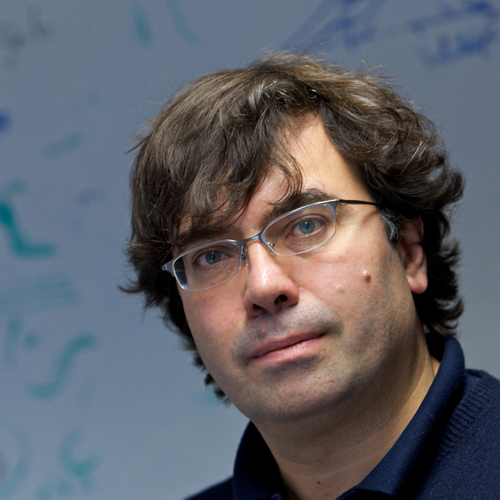
\includegraphics[height = 0.3\paperheight]{photos/nicola_marzari.jpg}  &
         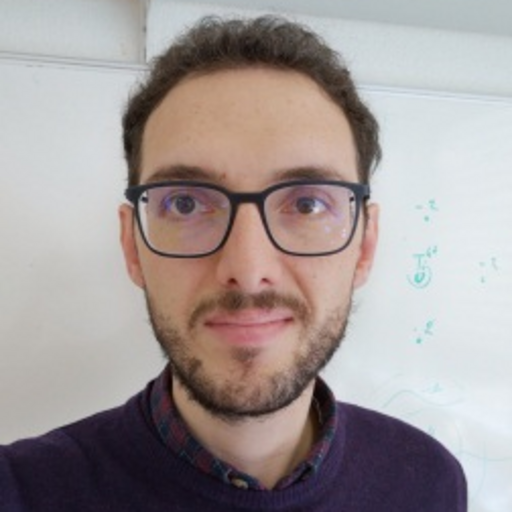
\includegraphics[height = 0.3\paperheight]{photos/nicola_colonna.png} \\
         Nicola Marzari                                                          &
         Nicola Colonna                                                          
      \end{tabularx}
   \end{center}
   \begin{center}
      
\includegraphics[height = 0.15\paperheight]{logos/snf_color.eps}
      \hspace{3em}
      
\includegraphics[height = 0.15\paperheight]{logos/marvel_color_on_white_trimmed.png}
   \end{center}

   \vspace{1ex}

   \begin{center}
      Want to find out more? Go to \textbf{\texttt{\href{https://koopmans-functionals.org/en/latest/}{koopmans-functionals.org}}}

      \vspace{1em}
      Follow 
\includegraphics[height=\fontcharht\font`\B]{logos/twitter.png} \textcolor{twitter_blue}{@ed\_linscott} for updates | Slides available at 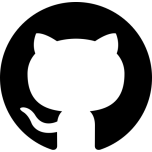
\includegraphics[height=\fontcharht\font`\B]{logos/github.png} \href{https://github.com/elinscott-talks/}{\textbf{\texttt{github/elinscott-talks}}}
   \end{center}

\end{frame}
\endgroup

% Backup slides
\backupbegin
\begin{frame}{}

   \begin{center}
      \huge SPARE SLIDES
   \end{center}

\end{frame}


\begin{frame}{Koopmans functionals: off-diagonal occupancies}
   \begin{block}{Recap from earlier}
      Key idea: construct a functional such that the \emph{variational} orbital energies
      \begin{equation*}
         \varepsilon^\mathsf{Koopmans}_i = \braopket{\varphi_i}{H}{\varphi_i} = \partial E_\mathsf{Koopmans}/\partial f_i
      \end{equation*}
      are...
      \begin{itemize}
         \item independent of the corresponding occupancies $f_i$
         \item equal to the corresponding total energy difference $E_i(N-1) - E(N)$
      \end{itemize}
   \end{block}

   zero band gap $\rightarrow$ occupancy matrix for variational orbitals is off-diagonal
\end{frame}


% \begin{frame}{References}
%    \setbeamercolor*{bibliography entry title}{fg=black}
%    \setbeamercolor*{bibliography entry author}{fg=black}
%    \setbeamercolor*{bibliography entry location}{fg=black}
%    \setbeamercolor*{bibliography entry note}{fg=black}
%    \printbibliography
%    % For further reading on Koopmans functionals, see \cite{Dabo2010,Borghi2014,Nguyen2018,Colonna2018,Colonna2019,DeGennaro2022,Colonna2022}
% 
% \end{frame}

\begin{frame}{Koopmans functionals: results for solids}
   \vspace{-0.5em}
   \begin{figure}[t]
      \centering
      \begin{subfigure}{0.45\textwidth}
         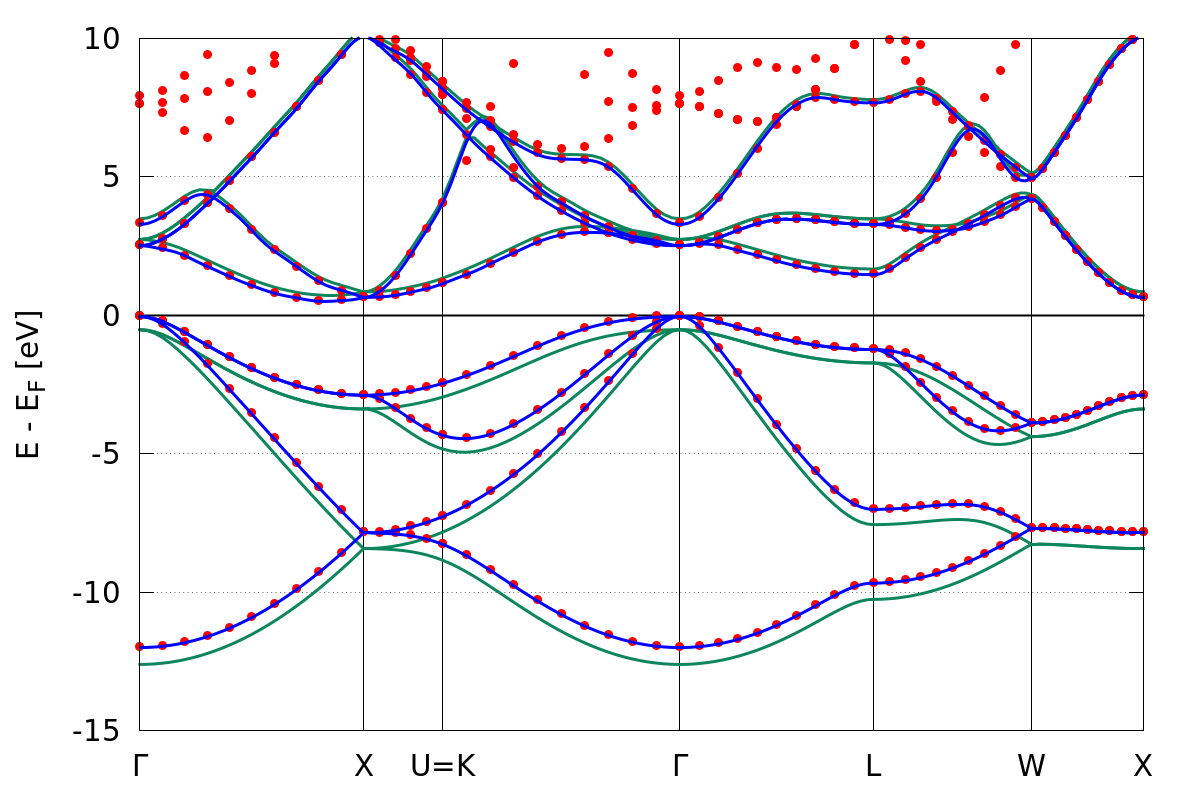
\includegraphics[width=\columnwidth]{figures/Si_kipz_bands.png}
         \caption{Si, KIPZ}
      \end{subfigure}
      \begin{subfigure}{0.45\textwidth}
         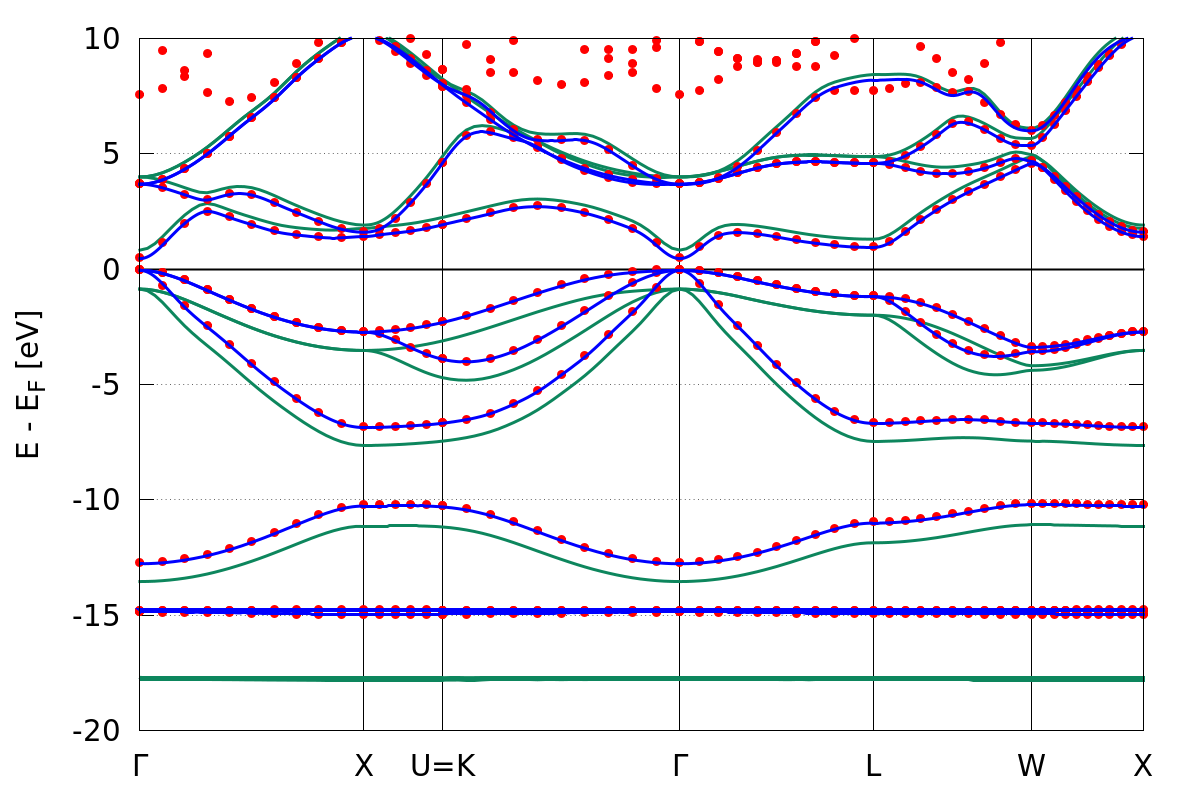
\includegraphics[width=\columnwidth]{figures/GaAs_ki_bands.png}
         \caption{GaAs, KI}
      \end{subfigure}
      % \begin{subfigure}{\textwidth}
      %    \begin{tabularx}{\columnwidth}{C C C C C C C}
      %       ZnO                                  & LDA  & HSE  & GW$_0$ & scG$\tilde{\rm W}$ & KI   & exp.      \\
      %       \hline
      %       $E_\mathsf{gap}$ (eV)                & 0.79 & 2.79 & 3.0    & 3.2                & 3.62 & 3.60      \\
      %       $\langle \varepsilon_d \rangle$ (eV) & -5.1 & -6.1 & -6.4   & -6.7               & -6.9 & -7.5/-8.0 \\
      %    \end{tabularx}
      % \end{subfigure}
   \end{figure}
   \begin{center}
      \footnotesize
      \begin{tabular}{l l S[table-format = 2.2] S[table-format = 2.2] >{\color{seaborn_red}\bfseries}S[table-format = 2.2] >{\color{seaborn_red}\bfseries}S[table-format = 2.2] >{\color{seaborn_red}\bfseries}S[table-format = 2.2] S[table-format = 2.2]}
                               &                                  & {PBE} & {QSG$\tilde{\mathsf{W}}$} & {KI} & {pKIPZ} & {\bf KIPZ} & {exp} \\
         \midrule
         \midrule
         {Si}                  & $E_\mathsf{gap}$                 & 0.55  & 1.24                      & 1.18 & 1.17    & 1.19       & 1.17  \\
         \midrule
         \multirow{2}{*}{GaAs} & $E_\mathsf{gap}$                 & 0.50  & 1.61                      & 1.53 & 1.49    & 1.50       & 1.52  \\
                               & $\langle \varepsilon_d \rangle $ & 14.9  & 17.6                      & 16.9 &         & 17.7       & 18.9
      \end{tabular}
   \end{center}
   \blfootcite{DeGennaro2022}
\end{frame}

\begin{frame}{Koopmans functionals: results for solids}
   \begin{figure}[t]
      \centering
      \begin{subfigure}{0.3\textwidth}
         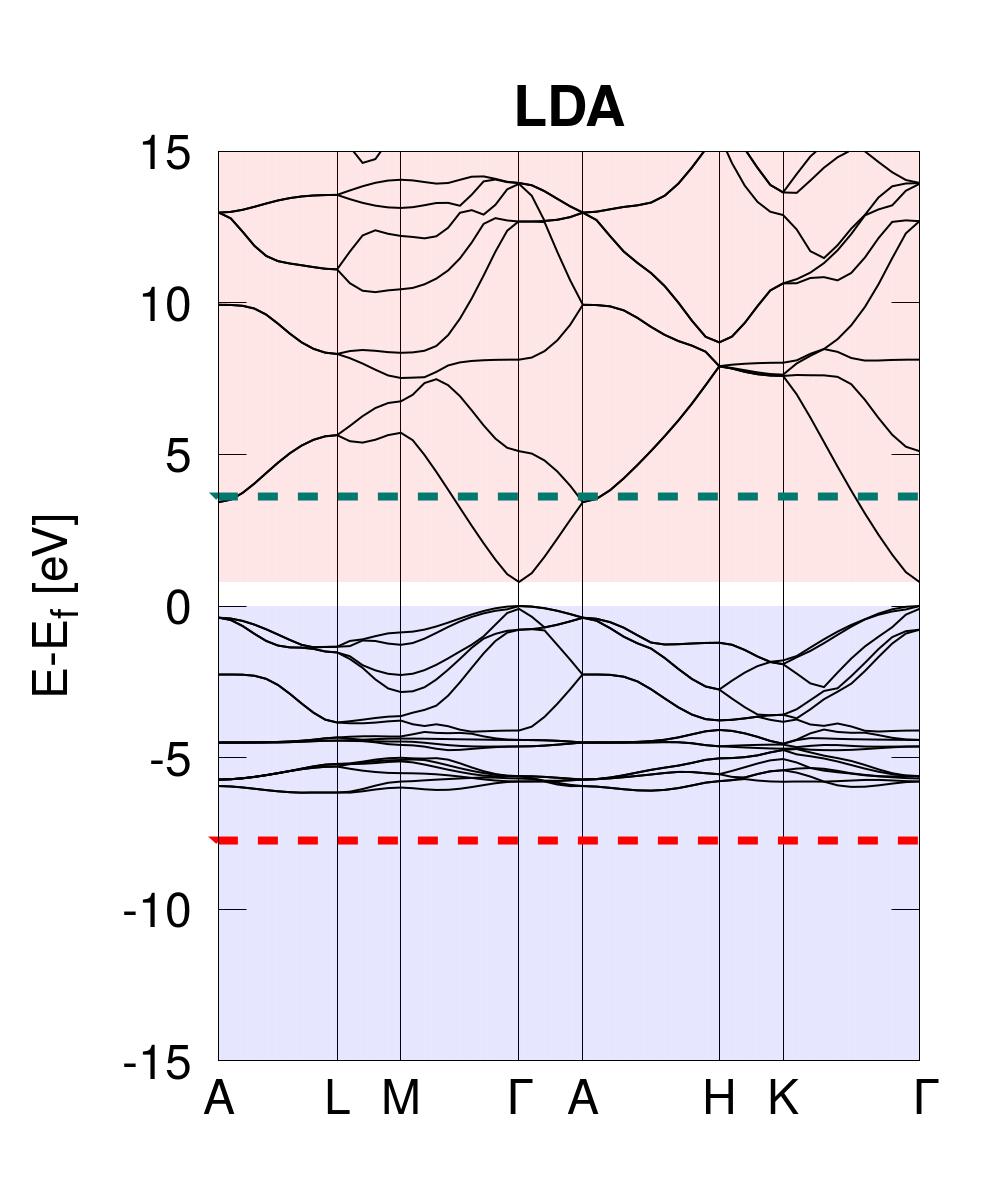
\includegraphics[width=\columnwidth]{figures/ZnO_lda.png}
      \end{subfigure}
      \begin{subfigure}{0.3\textwidth}
         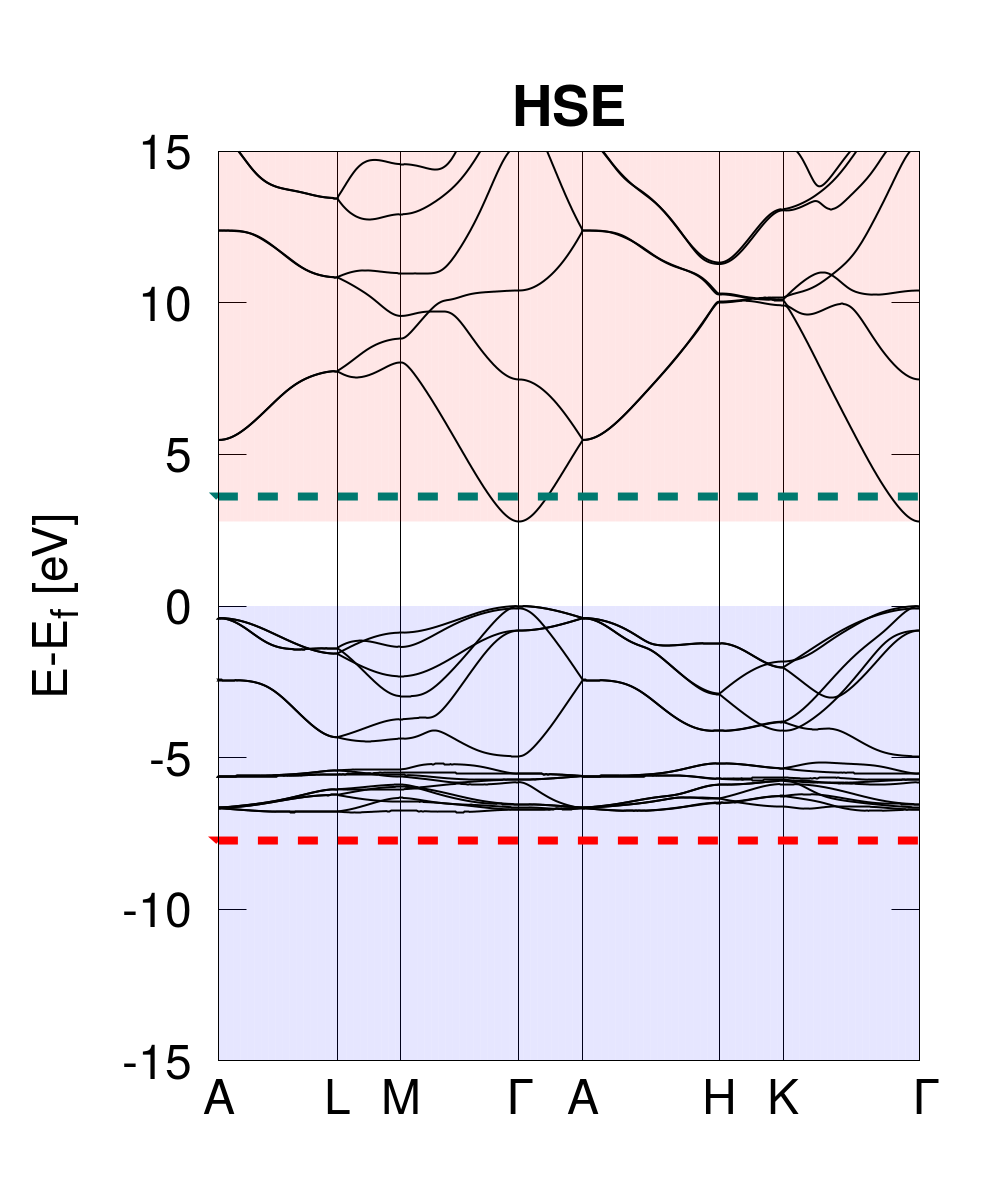
\includegraphics[width=\columnwidth]{figures/ZnO_hse.png}
      \end{subfigure}
      \begin{subfigure}{0.3\textwidth}
         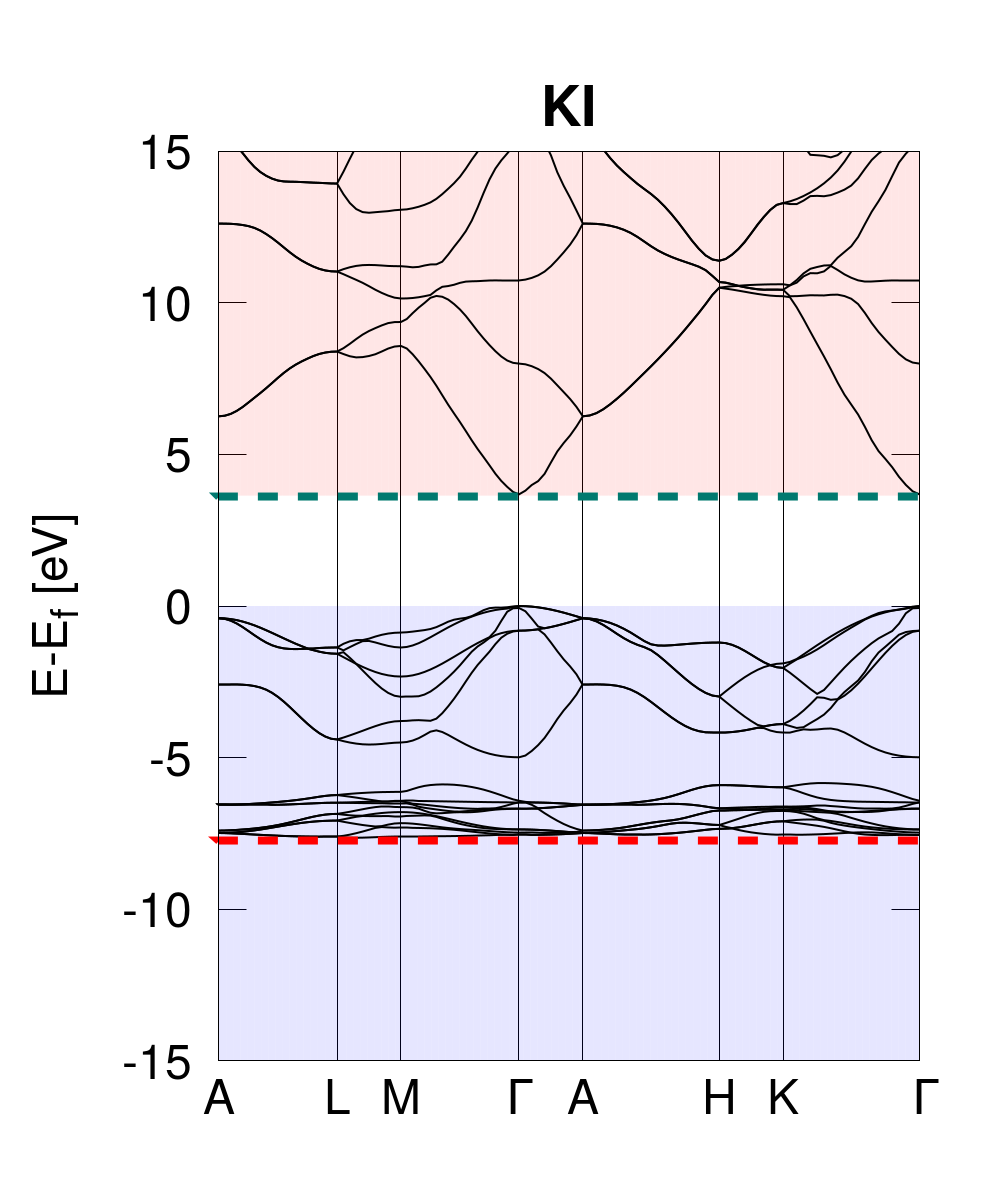
\includegraphics[width=\columnwidth]{figures/ZnO_ki.png}
      \end{subfigure}
      \begin{subfigure}{\textwidth} %<-- changed width
         \centering
         %    \renewcommand\tabularxcolumn[1]{m{#1}}% <-- added
         %    \renewcommand\arraystretch{1.3}
         %    \setlength\tabcolsep{2pt}% <-- added
         \begin{tabular}{c S[table-format = 2.2] S[table-format = 2.2] S[table-format = 2.2] S[table-format = 2.2] >{\color{seaborn_red}\bfseries}S[table-format = 2.2] S[table-format = 2.2]}
            ZnO                                  & {LDA} & {HSE} & {GW$_0$} & {scG$\tilde{\mathsf{W}}$} & {KI} & {exp}       \\
            \hline
            $E_\mathsf{gap}$ (eV)                & 0.79  & 2.79  & 3.0      & 3.2                  & 3.62 & 3.60        \\
            $\langle \varepsilon_d \rangle$ (eV) & -5.1  & -6.1  & -6.4     & -6.7                 & -6.9 & {-7.5/-8.0} \\
         \end{tabular}
         %        \caption{table}
      \end{subfigure}
      % \caption{Band structure of ZnO calculated at different level of theory:
      %    LDA (left panel), HSE (middle panel) and KI (right panel). Shaded areas
      %    highlight valence (light blue) and conduction (light red) manifolds. The
      %    experimental values for the band gap and for the energy position of
      %    Zn $d$-states are represented by the dashed green line and by the dashed
      %    red line, respectively.
      %    Table: Band gap and position of Zn $d$ states with respect to the top of the valence band at different level of theory compared to experimental and GW results from Ref.~\onlinecite{shishkin_accurate_2007}.}
   \end{figure}
   \blfootcite{Colonna2022}
\end{frame}

\begin{frame}{Accelerating improvements: screening via ML}
   \begin{center}
      \begin{tikzpicture}
         \node[inner sep=0pt] (water box) at (0,0)
         {
            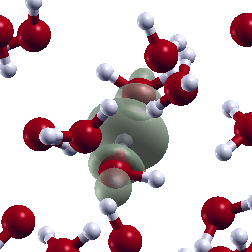
\includegraphics[width=0.25\textwidth]{figures/orbital_emp_00191_cropped.png}
         };
         \node[below=0cm of water box] (density) {$\rho_i(\mathbf{r})$};
         \node[right=0.2\textwidth of water box] (power spectrum) {
            $
               \begin{bmatrix}
                  x_{0} \\
                  x_{1} \\
                  x_{2} \\
                  \vdots
               \end{bmatrix}
            $
         };
         \path[line] (water box) -- node [midway, above, align=center] (decomposition) {power spectrum \\ decomposition} (power spectrum);
         \node[right=0.2\textwidth of power spectrum] (screening parameter) {$\alpha_i$};
         \path[line] (power spectrum) -- node [midway, above, align=center] (model) {ML model} (screening parameter);
      \end{tikzpicture}
   \end{center}

   \vspace{-4em}

   \blfootcite{Schubert2022}

   \begin{align*}
      c^i_{nlm,k} & =\int d\textbf{r} g_{nl}(r)Y_{lm}(\theta,\varphi)\rho^i(\textbf{r}-\textbf{R}^i)                        \\
      p^i_{n_1n_2l,k_1k_2}         & =\pi \sqrt{\frac{8}{2l+1}}\sum\limits_m {c_{n_1lm,k_1}^{i *}}c_{n_2lm,k_2}^i \label{eq: power spectrum}
   \end{align*}

   % $g_{nl}$ = orthonormalised radial Gaussian basis functions

   % $Y_{lm}$ = spherical harmonics

\end{frame}


\begin{frame}{Recent improvements: screening via ML}
   \begin{center}

      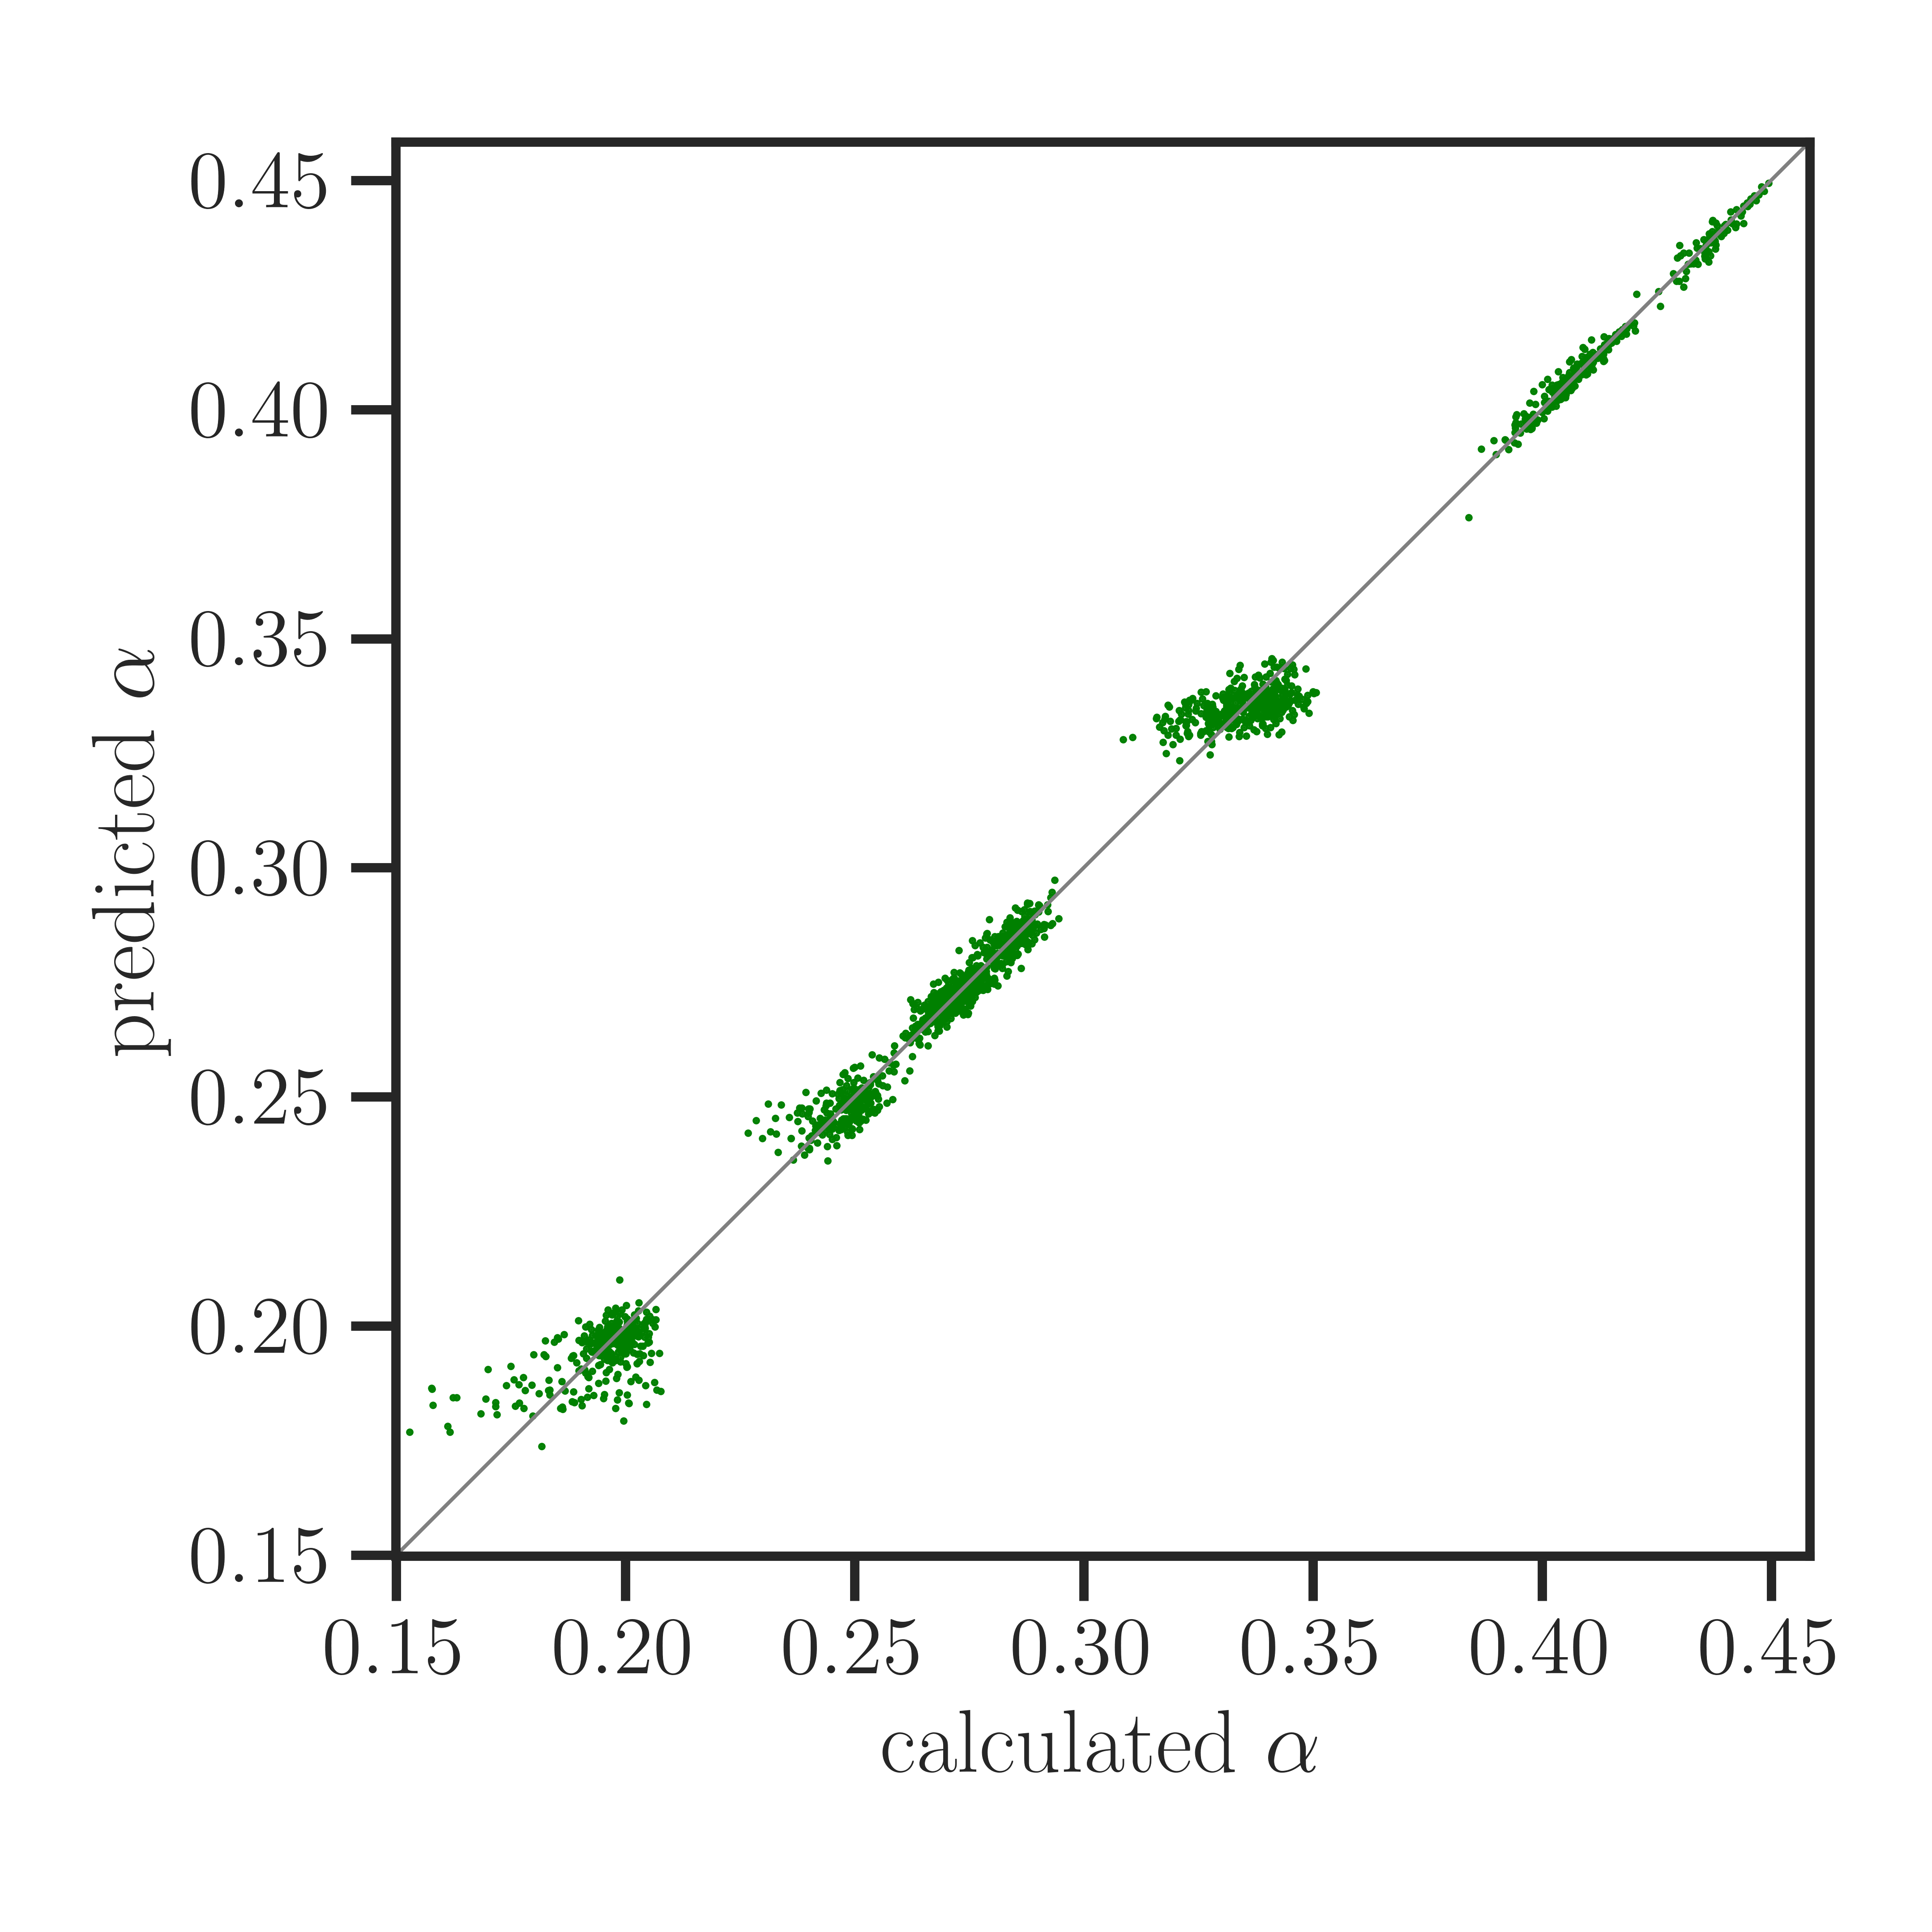
\includegraphics[height=0.7\paperheight]{figures/CsSnI3_calc_vs_pred_Edward.png}
      \includegraphics[height=0.7\paperheight]{figures/convergence_analysis_Edward.png}

      loss of accuracy of the band gap of $\sim$ 0.02 eV

      (cf. when calculating screening parameters \emph{ab initio})

      speedup of 70$\times$
   \end{center}

   \blfootcite{Schubert2022}

\end{frame}

\begin{frame}{Koopmans functionals: results for toy systems}
   Hooke's atom (two electrons in a harmonic confining potential)

   \begin{figure}[t]
      \begin{subfigure}{0.4\textwidth}
         \includegraphics[width=\columnwidth]{figures/schubert_vxc.jpeg}
      \end{subfigure}
      \begin{subfigure}{0.4\textwidth}
         \onslide<2->{
         \includegraphics[width=\columnwidth]{figures/schubert_vxc_integrated.jpeg}
         }
      \end{subfigure}
   \end{figure}

   \vspace{-4ex}

   \blfootcite{Schubert2023}
\end{frame}

\backupend
\end{document}
